%%%%%%%%%%%%%%%%%%%%%%%%%%%%%%%%%%%%%%%%%%%%%%%%%%%%%
%% File: main.tex
%% Author: Evangelos Stamos (estamos@e-ce.uth.gr)
%% Last update: January, 2020
%% Description: Provides an example of a Diploma Thesis 
%% using the ntua-thesis pdfLaTeX class.
%%
%% Character encoding: UTF-8
%%%%%%%%%%%%%%%%%%%%%%%%%%%%%%%%%%%%%%%%%%%%%%%%%%%%%
%
%
%%%%%%
% 1. use the "modern" or "classic" option to switch between 
% a modern or classic font, respectively.
%
% 2. add/remove the "hyperref" option to enable/disable hyperlinks:
% (remember to remove auxiliary files after adding/removing 
% the "hyperref" option).
%
% 3. add/remove the "printer" option to typeset a printer-friendly 
% (grayscale)/color version of the thesis.
%
% 4. use the "watermark" option to indicate that this is not an actual
% thesis.
%
% 5. use the "histinit" option to enable "historiated initials".
% (If used, all chapter initials declared by the \InitialCharacter{}
% macro are enlarged. If omitted, arguments of \InitialCharacter{}
% are typeset as normal text.)
%
% 6. use the "plain" option to disable tikz graphics in title page
% and part/chapter headers (might help to avoid compilation timeouts).
% Note that "plain" disables CD label and CD cover creation.
%
% 7. use the "noindex" option to (hopefully) avoid compilation timeouts
% when compiling online (disables index generation - note that "\indexGR",
% "\indexEN" invocations need not be removed when toggling this option).
%
% 8. activate the "newlogo" option to use the new official Logo.
%
%%%%%%%%%%%%%%%%%%%%%%%%%%%%%%%%%%%%%%%%%%%%%%%%%%%%%%%%%%%%%%%%%%%%%%%%%%%%%%%
%
\documentclass[modern,printer,hyperref,noindex,plain,newlogo]{ntua-thesis}
%
%%%%%%%%%%%%%%%%%%%%%%%%%%%%%%%%%%%%%%%%%%%%%%%%%%%%%%%%%%%%%%%%%%%%%%%%%%%%%%%
%
%
%%%%%%%%%%%%%%%%%%%%%%%%%%%%%%%%%%%%%%%%%%%%%%%%%%%%
%% THESIS INFO 
%%%%%%%%%%%%%%%%%%%%%%%%%%%%%%%%%%%%%%%%%%%%%%%%%%%%
%
% ΤΙΤΛΟΣ ΔΙΠΛΩΜΑΤΙΚΗΣ ΕΡΓΑΣΙΑΣ 
%
% Για εξαναγκασμένες αλλαγές γραμμής χρησιμοποιήστε "\\".
% Αν οι αλλαγές γραμμής πρέπει να είναι διαφορετικές στο εξώφυλλο σε σχέση 
% με το εσώφυλλο (σελ. 3), επαναλάβετε τον τίτλο του εξωφύλλου με τις 
% επιθυμητές αλλαγές γραμμής ως προαιρετικό όρισμα της εντολής \title.
%
% Παραδείγματα:
% 1. Όμοιος τίτλος σε εξώφυλλο και εσώφυλλο, με αυτόματες αλλαγές γραμμής:
%	    \title{Πρότυπο Σύστημα Ομότιμων Κόμβων Βασισμένο σε Σχήματα \en{RDF}}
% 2. Όμοιος τίτλος σε εξώφυλλο και εσώφυλλο, με αλλαγή γραμμής μετά τη λέξη
% "Σύστημα":
%	    \title{Πρότυπο Σύστημα \\ Ομότιμων Κόμβων Βασισμένο σε Σχήματα \en{RDF}}
% 3. Διαφορετικές αλλαγές γραμμής σε εξώφυλλο και εσώφυλλο. Στο εξώφυλλο 
% έχουμε αλλαγή γραμμής μετά τη λέξη "Σύστημα", ενώ στο εσώφυλλο η αλλαγή
% γραμμής ακολουθεί τη λέξη "Ομότιμων":
%	    \title[Πρότυπο Σύστημα \\ Ομότιμων Κόμβων Βασισμένο %
%           σε Σχήματα \en{RDF}]% (προαιρετικό όρισμα)
%           {Πρότυπο Σύστημα Ομότιμων \\ Κόμβων Βασισμένο σε %
%           Σχήματα \en{RDF}}% (υποχρεωτικό όρισμα)
%
	\title{Επιτάχυνση συνελικτικών νευρωνικών δικτύων με τεχνικές Παράλληλου Προγραμματισμού \\σε κάρτα γραφικών}
%%
%%
%
%% -------------------------------------------------------------------
%% ΥΠΟΤΙΤΛΟΣ ΔΙΠΛΩΜΑΤΙΚΗΣ ΕΡΓΑΣΙΑΣ (προαιρετικός)
%
% Αν δεν υπάρχει υπότιτλος, τοποθετήστε τον χαρακτήρα του σχολίου "%"
% πριν από την εντολή \subtitle, ή αφήστε κενό το όρισμα της εντολής.
%
% Παράδειγμα:
%%	\subtitle{Μελέτη και υλοποίηση}
	% \subtitle{Μελέτη και υλοποίηση}
%
%% -------------------------------------------------------------------
%% ΤΟΥ/ΤΗΣ/ΤΩΝ
%
% "του" ή "της" ή "των", ανάλογα με το φύλο/αριθμό του σπουδαστή ή 
% των σπουδαστών
% Παράδειγμα:
%	\toutis{του}
	\toutis{της}
     \foititi{φοιτήτριας}
%
%% -------------------------------------------------------------------
%% ΟΝΟΜΑΤΕΠΩΝΥΜΟ ΣΠΟΥΔΑΣΤΗ ΣΤΑ ΕΛΛΗΝΙΚΑ (ΚΕΦΑΛΑΙΑ, ΓΕΝΙΚΗ ΠΤΩΣΗ)
%
% Για περισσότερους του ενός σπουδαστές, διαχωρίστε με ",".
% Παράδειγμα:
%	\authorNameCapitalGR{ΚΩΝΣΤΑΝΤΙΝΟΥ Δ. ΔΗΜΗΤΡΙΟΥ, ΓΕΩΡΓΙΟΥ Π. ΠΑΝΑΓΑΚΗ}
	\authorNameCapitalGR{ΟΛΥΜΠΙΑΣ ΤΣΑΜΟΥ}
	\authorFatherCapitalGR{ΙΩΑΝΝΗ}
%
%% -------------------------------------------------------------------
%% ΟΝΟΜΑΤΕΠΩΝΥΜΟ ΣΠΟΥΔΑΣΤΗ ΣΤΗ ΛΑΤΙΝΙΚΗ ΜΟΡΦΗ (ΠΕΖΑ)
%
% Δηλώστε εδώ τυχόν ονοματεπώνυμα στη λατινική μορφή, αλλιώς αφήστε
% κενό το όρισμα.
% Για περισσότερους του ενός σπουδαστές, διαχωρίστε με ",".
% Παράδειγμα:
%	\authorNameEN{Albert Einstein, George W. Bush} 
	%\authorNameEN{Albert Einstein} 
%
%% -------------------------------------------------------------------
%% ΟΝΟΜΑΤΕΠΩΝΥΜΟ ΣΠΟΥΔΑΣΤΗ ΣΤΑ ΕΛΛΗΝΙΚΑ (ΠΕΖΑ, ΟΝΟΜΑΣΤΙΚΗ ΠΤΩΣΗ)
%
% Για περισσότερους του ενός σπουδαστές, διαχωρίστε με ",".
% Αν τα ονοματεπώνυμα όλων των σπουδαστών είναι σε λατινική μορφή,
% αφήστε κενό το όρισμα.
% Παράδειγμα:
%	\authorNameGR{Κωνσταντίνος Δημητρίου, Γεώργιος Παναγάκης}
	\authorNameGR{Ολυμπία Τσάμου}
%
%% -------------------------------------------------------------------
%% ΟΝΟΜΑΤΕΠΩΝΥΜΟ ΕΠΙΒΛΕΠΟΝΤΑ ΚΑΘΗΓΗΤΗ
% 
	\supervisor{Ευάγγελος Δερματάς}
%
%% -------------------------------------------------------------------
%% ΤΙΤΛΟΣ ΕΠΙΒΛΕΠΟΝΤΑ ΚΑΘΗΓΗΤΗ
%
	\supervisorTitle{Αναπληρωτής Καθηγητής}
%
%% -------------------------------------------------------------------
%% ΕΠΙΒΛΕΠΩΝ/ΕΠΙΒΛΕΠΟΥΣΑ
%
% "Επιβλέπων" ή "Επιβλέπουσα", ανάλογα με το φύλο του 
% Επιβλέποντα Καθηγητή
	\supervisorMaleFemale{Επιβλέπων}
%
%% -------------------------------------------------------------------
%% ΤΟΠΟΣ/ΜΗΝΑΣ/ΕΤΟΣ ΕΚΔΟΣΗΣ
%
	\thesisPlaceDate{Πάτρα, Ιούλιος 2024}
%
%% -------------------------------------------------------------------
%% ΤΟΠΟΣ/ΜΗΝΑΣ/ΕΤΟΣ ΣΥΓΓΡΑΦΗΣ (Εμφανίζεται στη σελίδα των ευχαριστιών,
%% αν υπάρχει).
%
	\ackPlaceDate{Πάτρα, Ιούλιος 2024}
%
%% -------------------------------------------------------------------
%% ΗΜΕΡΟΜΗΝΙΑ ΕΞΕΤΑΣΗΣ
%
	\examinationDate{?? / 07 / 2024}
%% -------------------------------------------------------------------
%% ΗΜΕΡΟΜΗΝΙΑ ΔΗΛΩΣΗΣ ΠΕΡΙ ΜΗ ΛΟΓΟΚΛΟΠΗΣ
%
	\declarationDate{?? Ιουλίου 2024}
%
%% -------------------------------------------------------------------
%% ΕΤΟΣ COPYRIGHT
%
	\copyrightYear{2024}
%
%% -------------------------------------------------------------------
%% ΟΝΟΜΑΤΕΠΩΝΥΜΟ 1ου ΕΞΕΤΑΣΤΗ
%
	\firstExaminer{Θεόδωρος Αντωνακόπουλος}
%
%% -------------------------------------------------------------------
%% ΤΙΤΛΟΣ 1ου ΕΞΕΤΑΣΤΗ
%
	\firstExaminerTitle{Καθηγητής}
%
%% -------------------------------------------------------------------
%% ΟΝΟΜΑΤΕΠΩΝΥΜΟ 2ου ΕΞΕΤΑΣΤΗ
%
	\secondExaminer{Σταύρος Κουλουρίδης}
%
%% -------------------------------------------------------------------
%% ΤΙΤΛΟΣ 2ου ΕΞΕΤΑΣΤΗ
%
	\secondExaminerTitle{Αναπληρωτής Καθηγητής}
%%
%%
%%%%%%%%%%%%%%%%%%%%%%%%%%%%%%%%%%%%%%%%%%%%%%%%%%%%%%%%%%%%%%%%%%%%%%
%% THESIS COLORS: 
%%%%%%%%%%%%%%%%%%%%%%%%%%%%%%%%%%%%%%%%%%%%%%%%%%%%%%%%%%%%%%%%%%%%%%
%%
%% Χρώμα εξωφύλλου - κεφαλαίων
	\chaptercolor{gray!50!brown}
%%
%% Χρώμα παραρτημάτων
	\appendixcolor{brown!60!orange}
%%
%% Χρώμα υπερσυνδέσμων (αν έχει ενεργοποιηθεί η επιλογή "hyperref")
    \hyperlinkcolor{blue}
%%
%% Χρώμα τίτλου εργασίας στο εξώφυλλο (αν δεν έχει ενεργοποιηθεί 
%% η επιλογή "plain")
    \titlecolor{white}
%%
%% Χρώμα υποβάθρου (φόντου) τίτλου εργασίας στο εξώφυλλο (αν δεν έχει 
%% ενεργοποιηθεί η επιλογή "plain")
    \titlebackgroundcolor{gray!60!brown}  
%%
%%
%%%%%%%%%%%%%%%%%%%%%%%%%%%%%%%%%%%%%%%%%%%%%%%%%%%%%%%%%%%%%%%%%%%%%%
%% COVER PAGE IMAGE: 
%%%%%%%%%%%%%%%%%%%%%%%%%%%%%%%%%%%%%%%%%%%%%%%%%%%%%%%%%%%%%%%%%%%%%%
%%
%% Εικόνα εξωφύλλου (προαιρετική)
%% Στην περίπτωση κατά την οποία δεν είναι επιθυμητή η εισαγωγή εικόνας στο εξώφυλλο,
%% διαγράψτε την εντολή \coverpageimage, ή μετατρέψτε την σε σχόλιο (με "%")
%%
%% Σύνταξη:
%%          \coverpageimage{συντελεστής μεγέθυνσης}{όνομα αρχείου εικόνας [πλήρης διαδρομή]}
%%      ή
%%          \coverpageimage[tikz]{συντελεστής μεγέθυνσης}{εντολές TikZ}
%%          (στις εντολές μπορούν να περιλαμβάνονται και δηλώσεις \usetikzlibrary, κ.λπ.)
%%      
%% Παραδείγματα:
%%      - Χρήση εικόνας από το αρχείο "figures/rdf.png" με συντελεστή μεγέθυνσης 0.8:
%%          \coverpageimage{0.8}{figures/rdf.png}
%%      - Χρήση εικόνας TikZ με συντελεστή μεγέθυνσης 0.5:
%%          \coverpageimage[tikz]{0.5}{
%%              \draw[thick, gray] \foreach \x in {18,90,...,306} {
%%                  (\x:4) node{} -- (\x+72:4)
%%                  (\x:4) -- (\x:3) node{}
%%                  (\x:3) -- (\x+15:2) node{}
%%                  (\x:3) -- (\x-15:2) node{}
%%                  (\x+15:2) -- (\x+144-15:2)
%%                  (\x-15:2) -- (\x+144+15:2)
%%              };
%%          }
%%
     % \coverpageimage{0.8}{figures/rdf.png}
%%
%%%%%%%%%%%%%%%%%%%%%%%%%%%%%%%%%%%%%%%%%%%%%%%%%%%%%%%%%%%%%%%%%%%%%%
%
% add custom hyphenation rules here
\hyphenation{ο-ποί-α} 
%
%%%%
%
%
%%%%
\begin{document}

\maketitle

\beginfrontmatter
	
% Περίληψη
	\begin{abstract}
Στην παρούσα εργασία θα αξιολογηθεί η βελτιστοποίηση της ταχύτητας εκτέλεσης ενός συνελικτικού νευρωνικού δικτύου, το οποίο ταξινομεί εικόνες, μετατρέποντας τον κώδικα σε παράλληλο ώστε να εκμεταλλευτούμε την υπολογιστική ισχύ μιας κάρτας γραφικών. Πιο συγκεκριμένα, αρχικά θα γίνει αναφορά στα νευρωνικά δίκτυα, εστιάζοντας στα συνελικτικά νευρωνικά δίκτυα και πώς αυτά χρησιμοποιούνται στην αναγνώριση εικόνων. Σε επόμενο κεφάλαιο, θα εξεταστεί η χρήση του παράλληλου προγραμματισμού και της υπολογιστικής υψηλής απόδοσης σήμερα. Επιπλέον, θα αναφερθούμε στα μοντέλα παράλληλου προγραμματισμού για \tl{CPU} και στη χρήση των \tl{GPU} για επιτάχυνση της εκτέλεσης υπολογιστικά κοστοβόρων προβλημάτων. Ιδιαίτερη έμφαση δίνεται στην \tl{OpenACC} για την παραλληλοποίηση και βελτιστοποίηση κώδικα σε επιταχυντές, όπως οι \tl{GPU}. Τέλος, προσθέτοντας τις κατάλληλες εντολές σε έναν σειριακό κώδικα ταξινόμησης εικόνων ώστε να τρέχει παράλληλα σε μια κάρτα γραφικών, θα γίνει σύγκριση των χρόνων εκτέλεσης των προγραμμάτων και ανάλυση των αποτελεσμάτων που θα εξαχθούν.

   \begin{keywords}
   Ταξινόμηση εικόνων, Συνελικτικά Νευρωνικά Δίκτυα, Παράλληλος Προγραμματισμός, Κάρτες Γραφικών, \tl{OpenACC}
   \end{keywords}
\end{abstract}



\begin{abstracteng}
\tl{In this thesis, we evaluate the optimisation of execution speed in a convolutional neural network for image classification by parallelising its code to leverage the computational power of a graphics card. We begin by discussing neural networks, focusing on convolutional neural networks and their application in image recognition. In the next chapter, we explore the current use of parallel programming and high-performance computing. Furthermore, we discuss parallel programming models for CPUs and the use of GPUs to accelerate computationally intensive tasks, with a particular focus on OpenACC for parallelising and optimising code on accelerators such as GPUs. Finally, by adding the appropriate instructions to serial image classification code to enable parallel execution on a graphics card, we compare the execution times of the programmes and analyse the results.}

   \begin{keywordseng}
    \tl{Image Classification, Convolutional Neural Networks, Parallel Computing, GPU, OpenACC}
   \end{keywordseng}

\end{abstracteng}
% % Αφιέρωση
% 	\thesisDedication{στους γονείς μου}
% % Ευχαριστίες
% 	%%%%%%%%%%%%%%%%%%%%%%%%%%%%%%%%%%%%%%%%%%%%%%%%%%%%%%%%%%%%%%%%%
%%
%% use the starred version of the "acknowledgements" environment
%% to omit signatures from this section, e.g.:
%% \begin{acknowledgements*} ... \end{acknowledgements*}
%% 
%%%%%%%%%%%%%%%%%%%%%%%%%%%%%%%%%%%%%%%%%%%%%%%%%%%%%%%%%%%%%%%%%
\begin{acknowledgements}
Θα ήθελα καταρχήν να ευχαριστήσω τον καθηγητή κ. .........
για την επίβλεψη αυτής της διπλωματικής εργασίας και για την
ευκαιρία που μου έδωσε να την εκπονήσω στο εργαστήριο Συστημάτων
Βάσεων Γνώσεων και Δεδομένων. Επίσης ευχαριστώ ιδιαίτερα τον Δρ.
............ για την καθοδήγησή του και την εξαιρετική
συνεργασία που είχαμε. Τέλος θα ήθελα να ευχαριστήσω τους γονείς
μου για την καθοδήγηση και την ηθική συμπαράσταση που μου
προσέφεραν όλα αυτά τα χρόνια.
\end{acknowledgements}
% Πίνακας Περιεχομένων
	\tableofcontents
% Κατάλογος Σχημάτων
	\listoffigures
% Κατάλογος Εικόνων
	\listofillustrations
% % Κατάλογος Πινάκων
% 	\listoftables
% % Πρόλογος
% 	\begin{preface}
Στον πρόλογο αναφέρονται θέματα που δεν είναι επιστημονικά ή τεχνικά, όπως το πλαίσιο που διενεργήθηκε η εργασία, ο τόπος διεξαγωγής, το Εργαστήριο στο οποίο εκπονήθηκε κ.λπ. 
\end{preface}
	
\beginmainmatter

%%%%%%%%%%%%%%%%%%%%%%%%%%%%%%%%%%%%%%%%%%%%%%%%%%%%%
%% INCLUDE YOUR CHAPTERS/SECTIONS HERE
%%
% Εισαγωγή
	\chapter{Εισαγωγή} 
Η τεχνητή νοημοσύνη και η βαθιά μάθηση \en{(deep learning)} έχουν διεισδύσει σε πολυάριθμες πτυχές της καθημερινής ζωής. Οι τεχνολογίες αυτές χρησιμοποιούνται ολοένα και περισσότερο, από την ιατρική και την επιστημονική έρευνα έως τις εφαρμογές επεξεργασίας εικόνας και αναγνώρισης ομιλίας, καθώς και τους προσωπικούς βοηθούς στα κινητά μας τηλέφωνα. Αυτό είναι δυνατό λόγω της αυξανόμενης ισχύος υπολογιστικών συστημάτων και αρχιτεκτονικών, οι οποίες επιτρέπουν την επεξεργασία μεγάλου όγκου δεδομένων. 

Τα νευρωνικά δίκτυα, και ειδικότερα τα συνελικτικά νευρωνικά δίκτυα (\en{CNN}) έχουν αποδειχθεί εξαιρετικά αποτελεσματικά στην ανάλυση και ταξινόμηση εικόνων με μεγάλη ακρίβεια. Η αποτελεσματικότητά τους προέρχεται από την πολύπλοκη αρχιτεκτονική τους. Τα νευρωνικά δίκτυα συνιστούν μια μαθηματική μοντελοποίηση του τρόπου λειτουργίας του ανθρώπινου εγκεφάλου και της διαδικασίας μάθησης. Ουσιαστικά, εκτελούν μια σειρά μετασχηματισμών δεδομένων και εφαρμογές συναρτήσεων με εκπαιδεύσιμες παραμέτρους, διαδικασία που περιλαμβάνει πολλές επαναλήψεις και μαθηματικούς υπολογισμούς. 

Ένας σημαντικός παράγοντας που συνέβαλε στην εξάπλωση των νευρωνικών δικτύων ήταν η εξέλιξη των καρτών γραφικών (\en{GPU}) και η χρήση τους για προγραμματισμό γενικού σκοπού. Καθώς η κατασκευή γρηγορότερων επεξεργαστών έφτασε στα όριά της, λόγω ζητημάτων που αφορούν την κατανάλωση ενέργειας και την έκλυση θερμότητας από την αύξηση της ταχύτητας του ρολογιού, η αύξηση της επεξεργαστικής ισχύος σήμερα επιτυγχάνεται μέσω της χρήσης πολλαπλών πυρήνων. Οι κάρτες γραφικών διαθέτουν εκατοντάδες έως χιλιάδες επεξεργαστικούς πυρήνες που μπορούν να εκτελούν εντολές παράλληλα, καταναλώνοντας λιγότερη ενέργεια σε σχέση με τις κεντρικές μονάδες επεξεργασίας (\en{CPU}). Επιπλέον, η πρόσβαση σε αυτές είναι εύκολη καθώς πλέον υπάρχουν σε προσωπικούς υπολογιστές και ενσωματωμένα συστήματα. Έτσι, οι κάρτες γραφικών χρησιμοποιούνται τόσο στη φάση της εκπαίδευσης (\en{training}) όσο και στη φάση της εξαγωγής συμπερασμάτων (\en{inference}), δίνοντας αποτελέσματα σε πραγματικό χρόνο.


\section{Αντικείμενο της διπλωματικής}
\en{?? }Η παρούσα εργασία έχει ως σκοπό την αξιολόγηση της βελτιστοποίησης της ταχύτητας εκτέλεσης ενός συνελικτικού νευρωνικού δικτύου που ταξινομεί εικόνες, χρησιμοποιώντας τεχνικές παράλληλου προγραμματισμού. 
Υλοποίηση σειριακού κώδικα του συνελικτικού νευρωνικού δικτύου που κάνει ταξινόμηση εικόνων.
Η υλοποίηση έγινε σε γλώσσα \en{C}.
Σύνολο δεδομένων που ταξινομείτε είναι το \en{CIFAR-10}.
Χρήση παράλληλου προγραμματισμού για βελτιστοποίηση της ταχύτητας.
Αξιοποίηση της επεξεργαστικής ισχύος μιας κάρτας γραφικών.
Για προγραμματισμό σε κάρτα γραφικών χρησιμοποιήθηκε το προγραμματιστικό πρότυπο \en{OpenACC}, η παραλληλοποίηση γίνεται με εισαγωγή εντολών προς τον μεταγλωττιστή, διατηρώντας τον σειριακό κώδικα.
Αυτό προσφέρει φορητότητα, επιτρέποντας την εκτέλεση ακόμη και σε συστήματα χωρίς συμβατές κάρτες γραφικών.

\en{??} Πολλές είναι οι εφαρμογές όπου η γρήγορη εκτέλεση της εξαγωγής συμπερασμάτων είναι σημαντική. Η πιο χαρακτηριστική είναι στην αυτόνομη οδήγηση. Τα συνελικτικά νευρωνικά δίκτυα χρησιμοποιούνται για την αναγνώριση αντικειμένων όπως πεζοί, άλλα οχήματα, σήματα οδικής κυκλοφορίας και εντοπισμός εμποδίων, απαιτώντας γρήγορους χρόνους αντίδρασης για την αποφυγή ατυχημάτων. Αντίστοιχες απαιτήσεις υπάρχουν στη ρομποτική, όπου η πλοήγηση και η αλληλεπίδραση με το περιβάλλον πραγματοποιούνται αναλύοντας εικόνες ή βίντεο και λαμβάνοντας σήματα από διάφορους αισθητήρες.\cite{Ilas2020}

Στην ιατρική, τα συνελικτικά νευρωνικά δίκτυα χρησιμοποιούνται για την ανάλυση ιατρικών εικόνων, όπως ακτινογραφίες, μαγνητικές τομογραφίες και αξονικές τομογραφίες. Μπορούν να ανιχνεύσουν ανωμαλίες και ασθένειες όπως όγκους, κατάγματα και λοιμώξεις, βοηθώντας τους γιατρούς στην ακριβή διάγνωση. \cite{Ilas2020}, \cite{McKinney2020}

Η πρόβλεψη του καιρού και αλλαγές στο κλίμα είναι ένας ακόμη τομέας όπου η ταχύτητα εκτέλεσης των συνελικτικών νευρωνικών δικτύων έχει κάνει την έγκυρη ενημέρωση εφικτή. Τα μοντέλα που έχουν αναπτυχθεί παρέχουν ακριβείς πληροφορίες που σχετίζονται με την καλλιέργεια γης, τη ρύθμιση δρομολογίων στις μεταφορές και κρίσιμες πληροφορίες για την πρόληψη και διαχείριση φυσικών καταστροφών. \cite{Chen2023}

\section{Οργάνωση του τόμου}
\en{??} Η εργασία αυτή είναι οργανωμένη σε επτά κεφάλαια: Στο Κεφάλαιο 2
δίνεται το θεωρητικό υπόβαθρο των βασικών τεχνολογιών που
σχετίζονται με τη διπλωματική αυτή. Αρχικά περιγράφονται τα νευρωνικά δίκτυα, στη συνέχεια τα συνελικτικά νευρωνικά δύκτυα ... . Στο
Κεφάλαιο 3 αρχικά περιγράφεται η παράλληλη επεξεργασία
.... . Στο Κεφάλαιο 4 παρουσιάζεται η υλοποίηση του κώδικα και η παραλληλοποιηση του ....
Τέλος στο Κεφάλαιο 5 δίνεται η συνεισφορά αυτής της
διπλωματικής εργασίας, καθώς και μελλοντικές επεκτάσεις.
% Μέρη/Κεφάλαια
	\part{Θεωρητικό Μέρος}
	\chapter{Θεωρητικό υπόβαθρο}
?? Στο κεφάλαιο αυτό παρουσιάζονται  αναλυτικά οι τρεις
βασικές τεχνολογίες που έχουν σχέση με την εργασία αυτή, δηλαδή ...

\section{Υπολογιστική Όραση}

Ο άνθρωπος βασίζεται στην αίσθηση της όρασης στην καθημερινή του ζωή. Ο τρόπος με τον οποίο αναλύουμε το περιβάλλον γύρω μας και παίρνουμε αποφάσεις γίνεται ασυναίσθητα. Η υπολογιστική όραση έχει στόχο την δημιουργία συστημάτων που μπορούν να πλοηγούνται στο ίδιο περιβάλλον με εμάς, κάνουν προβλέψεις και παίρνουν αποφάσεις με βάση εικόνες. Ο σχεδιασμός τέτοιων συστημάτων επιτυγχάνεται με αλγόριθμους βαθιάς μάθησης και μηχανικής μάθησης. Αυτοί οι αλγόριθμοι εκπαιδεύονται με μεγάλα σύνολα δεδομένων εικόνων, επιτρέποντας την αναγνώριση προτύπων, αντικειμένων και συνθήκες στο περιβάλλον γύρω τους.

Αν και η μηχανική μάθηση υπάρχει ως αντικείμενο εδώ και πολλά χρόνια, πρόσφατα έχει προσελκύσει έντονο ενδιαφέρον λόγω των σημαντικών προόδων που σημειώθηκαν στην υπολογιστική ισχύ και τη διαθεσιμότητα μεγάλου όγκου δεδομένων για εκπαίδευση.

Σήμερα, εφαρμογές της υπολογιστικής όρασης και των αλγορίθμων βαθιάς μάθησης συναντάμε σε πολλούς τομείς. Αρχικά, επιτρέπει στα ρομπότ να αντιλαμβάνονται οπτικά στοιχεία στο περιβάλλον τους, κρίσιμα για την πλοήγηση τους στον κόσμο μαζί με εμάς. Αλγόριθμους μηχανικής μάθησης και συστήματα τεχνητής νοημοσύνης συναντάμε ακόμη και στα κινητά μας τηλέφωνα. Εφαρμογές επεξεργασίας εικόνων, βελτίωσης των φωτογραφιών, ανίχνευση προσώπων και αναγνώριση κειμένου είναι μόνο μερικά από αυτά.

Ένας από τους πιο σημαντικούς τομείς εφαρμογής είναι η ιατρική, όπου από ιατρικές εικόνες εξάγονται πληροφορίες για τη διάγνωση ενός ασθενούς. Όπως για παράδειγμα η έγκυρη διάγνωση για καρκίνο του μαστού από μαστογραφίες ή ο εντοπισμός όγκου στον εγκέφαλο από μαγνητικές τομογραφίες.

Μια άλλη εφαρμογή της υπολογιστικής όρασης και των αλγόριθμων βαθιάς μάθησης είναι η αυτόνομή οδήγηση. Τα συστήματα αυτά αναγνωρίζουν σήματα, εμπόδια, πεζούς και άλλα οχήματα, αλλά κάνουν και προβλέψεις για την κίνηση αυτών και παίρνουν τις κατάλληλες αποφάσεις για ασφαλή πλοήγηση στους δρόμους.

\section{Πώς ένας υπολογιστής αναγνωρίζει εικόνες}

Ένα από τα βασικά προβλήματα στην Υπολογιστική Όραση είναι αυτό της ταξινόμησης εικόνων. Το πρόβλημα περιλαμβάνει την ανάθεση ετικέτας σε μια εικόνα εισόδου από ένα σταθερό σύνολο κατηγοριών.

Σε αντίθεση με έναν αλγόριθμο που ταξινομεί μια λίστα αριθμών, δεν είναι προφανής ο τρόπος υλοποίησης ενός αλγορίθμου που θα αναγνωρίζει εικόνες. Αντί να προσπαθούμε να προσδιορίσουμε τα χαρακτηριστικά της κάθε κατηγορίας με κώδικα, η προσέγγιση που ακολουθούμε μοιάζει με αυτή που θα ακολουθούσαμε με ένα παιδί. Δίνουμε στον υπολογιστή πολλά παραδείγματα κάθε κατηγορίας και στη συνέχεια αναπτύσσουμε αλγορίθμους μάθησης που εξετάζουν αυτά τα παραδείγματα και μαθαίνουν για την οπτική εμφάνιση κάθε κατηγορίας. Αυτή η προσέγγιση αναφέρεται ως προσέγγιση με βάση τα δεδομένα, καθώς πρώτα συλλέγει δεδομένα από ένα σύνολο κατηγοριοποιημένων δεδομένων.

\subsection{Τι είναι τα Νευρωνικά Δίκτυα?}
Τα νευρωνικά δίκτυα είναι αλγόριθμοι μηχανικής μάθησης εμπνευσμένοι από τον τρόπο λειτουργίας του ανθρώπινου εγκεφάλου. 

Ο εγκέφαλος περιέχει περισσότερα από 80 δισεκατομμύρια κύτταρα - που ονομάζονται νευρώνες - τα οποία ανταλλάσσουν πληροφορίες μεταξύ τους μέσω μικρών παλμών ηλεκτρισμού. Ένας νευρώνας δεν μιλάει απευθείας με όλους τους 80 δισεκατομμύρια άλλους. Αντίθετα, συνδέονται σε δομές που εκτελούν εξειδικευμένες λειτουργίες. Αυτές οι δομές είναι τα βιολογικά νευρωνικά δίκτυα.

Ο ανθρώπινος εγκέφαλος είναι πολύ περίπλοκος, όμως το πιο σημαντικό χαρακτηριστικό που μας ενδιαφέρει είναι η ικανότητα να μαθαίνει από την εμπειρία. Κάθε φορά που μαθαίνουμε κάτι καινούριο, οι νευρώνες στον εγκέφαλό ενισχύουν τις γραμμές επικοινωνίας τους με ορισμένους νευρώνες και αποδυναμώνουν τις συνδέσεις τους με άλλους. Η δομή ενός νευρωνικού δικτύου εξελίσσεται καθώς αποκτάμε νέες ικανότητες. [5]

\subsubsection{Νευρώνας}

Η βασική υπολογιστική μονάδα τον τεχνιτών νευρωνικών δικτύων είναι ο νευρώνας. Οι νευρώνες συνδέονται μεταξύ τους μέσω συνάψεων και σε κάθε σύναψη αντιστοιχεί ένα βάρος \(w_{ij}\), όπου \(j\) είναι ο νευρώνας που στέλνει το σήμα και \(i\) ο νευρώνας που δέχεται το σήμα. Τα σήματα εισόδου που φτάνουν σε έναν νευρώνα μέσω των συνάψεων, πολλαπλασιάζονται με το αντίστοιχο βάρος \(w_{ij}\) και αθροίζονται. Τα βάρη αποτελούν τα εκπαιδεύσιμα στοιχεία των νευρωνικών δικτύων και η τιμή τους έχει να κάνει με το πόσο ένας νευρώνας επηρεάζει έναν άλλο. Εάν το τελικό άθροισμα είναι πάνω από ένα όριο, ο νευρώνας ενεργοποιείται και στέλνει σήμα στην έξοδο. Αυτό μαθηματικά αναπαρίσταται με μία συνάρτηση ενεργοποίησης \(f\), με πιο συνηθισμένη τη σιγμοειδή $\sigma(x) ={1}/{(1 + e^{-x})}$, η οποία περιορίζει τις τιμές στο εύρος από \(0\) έως \(1\). [5]

\begin{Illustration}[!h] 
\centering
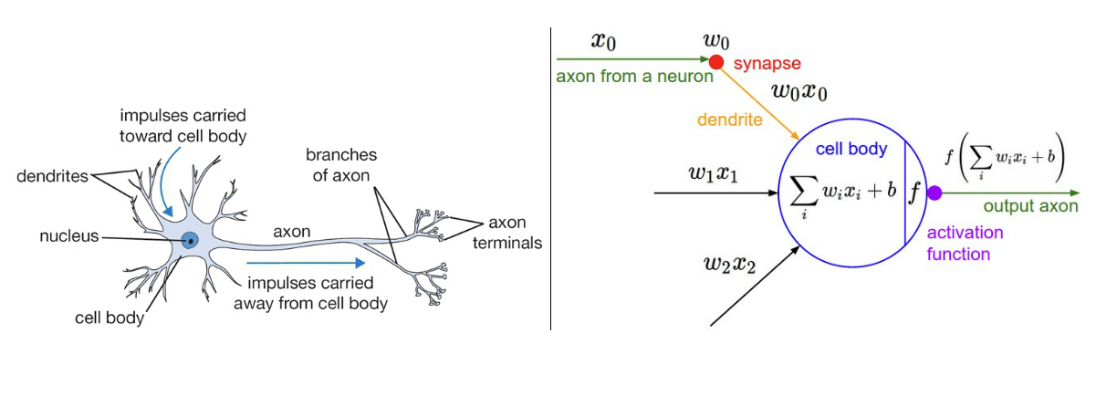
\includegraphics{images/image005.png} 
\caption{Βιολογική και μαθηματική απεικόνιση του νευρώνα [5]} 
\label{neuron-illustration}
\end{Illustration}

\noindent
\begin{minipage}{\textwidth}
\begin{equation}
\hat{x} = \mathbf{x} \mathbf{w} = \sum_{i=1}^{N} x_i w_i + b
\end{equation}

\begin{equation}
y = f(\hat{x})
\end{equation}
\end{minipage}

\subsubsection{Συναρτήσεις Ενεργοποίησης}
Η συνάρτηση ενεργοποίησης, είναι αυτή που εισάγει τη μη γραμμικότητα στο δίκτυο. Χωρίς αυτή ο νευρώνας συμπεριφέρεται σαν γραμμικός ταξινομητής. 

Τα χαρακτηριστικά που θέλουμε να έχει μια συνάρτηση ενεργοποίησης είναι να είναι αύξουσα, να έχει πεπερασμένα απειροστικά όρια, να έχει πεδίο ορισμού το σύνολο των πραγματικών αριθμών και φραγμένο πεδίο τιμών.[6]

Μερικά παραδείγματα συναρτήσεων ενεργοποίησης που συναντάμε φαίνονται παρακάτω:  
 \begin{Illustration}[!h] 
 \centering
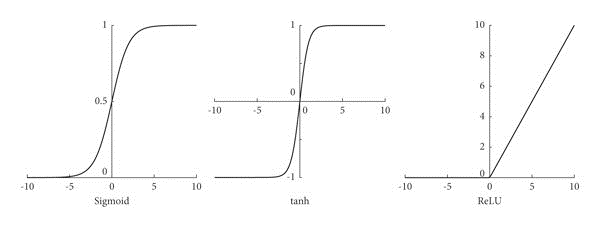
\includegraphics[width=\textwidth]{images/image008.png} \caption{Γραφικές παραστάσεις Σιγμοειδής, Υπερβολική Εφαπτομένη και  \en{ReLU} [7]} 
\label{fig:activation-functions}
\end{Illustration}
\begin{itemize}
\item Σιγμοειδής (\en{Sigmoid})

Η σιγμοειδής συνάρτηση $\sigma(x) ={1}/{(1 + e^{-x})}$, όπως αναφέρθηκε και παραπάνω φράσει την έξοδο ανάμεσα στο $0$ και $1$.  Χρησιμοποιείται συνήθως για μοντέλα όπου η έξοδος εκφράζει πρόβλεψη πιθανότητας. Το μειονέκτημα της  είναι πως ο νευρώνας μπορεί να κορεστεί στο $0$ ή στο $1$, με την παράγωγο να μηδενίζεται σε αυτές τις περιοχές, πράγμα που δημιουργεί πρόβλημα στην διαδικασία της εκπαίδευσης και χρειάζεται προσοχή στην αρχικοποίηση των βαρών. Επιπλέον, η σιγμοειδής δεν έχει κέντρο στο μηδέν, το οποίο μπορεί να προκαλέσει ανεπιθύμητη κίνηση ζιγκ-ζαγκ κατά τις ενημερώσεις των συντελεστών $w$.[5]
\item Υπερβολική εφαπτομένη –  \en{Tanh}

Η υπερβολική εφαπτομένη έχει πεδίο τιμών το $[-1,1]$. Όπως και στην σιγμοειδή, οι νευρώνες μπορεί να κορεστούν, όμως έχει κέντρο το $0$. 
\[
\tanh(x) = \frac{e^x - e^{-x}}{e^x + e^{-x}}
\]

\item Ανορθωμένη γραμμική συνάρτηση - \en{ReLU  (Rectified Linear Unit)}

Η \en{ReLU} όπως φαίνεται από τον τύπο, είναι ένα κατώφλι στο μηδέν
\[
f(x) = \max(0, x) = 
\begin{cases} 
x & \text{\en{if} } x \geq 0 \\
0 & \text{\en{if} } x < 0 
\end{cases}
\]
Χρησιμοποιείται στα νευρωνικά δίκτυα πολλών επιπέδων καθώς φαίνεται να επιταχύνει κατά πολύ την σύγκλιση του αλγόριθμου εκπαίδευσης στοχαστικής καθόδου με βάση την κλίση \en{(stochastic gradient descent)} σε σχέση με την υπερβολική εφαπτομένη και τη σιγμοειδή. Επιπλέον, στον υπολογισμό της είναι πολύ απλή σε σχέση με συναρτήσεις που περιέχουν εκθετικά. Το μειονέκτημα της είναι πώς η μηδενική πλευρά έχει παραγωγό 0 και κατά την εκπαιδεύσει μπορεί κάποιοι νευρώνες να μην ενεργοποιηθούν ποτέ.
\end{itemize}

\subsection{Δομή νευρωνικού δικτύου}
Τα Νευρωνικά δίκτυα οργανώνονται σε επίπεδα από νευρώνες. Ένα επίπεδο εισόδου, ένα ή παραπάνω ενδιάμεσα κρυφά επίπεδα, και ένα επίπεδο εξόδου [8]. Ο πιο συνηθισμένος τρόπος διασύνδεσης των επιπέδων είναι το πλήρως διασυνδεμένο επίπεδο, όπου κάθε νευρώνας συνδέεται με τους νευρώνες του επόμενου επιπέδου και οι έξοδοι των νευρώνων του ενός επιπέδου γίνονται είσοδος του επόμενου, χωρίς όμως να έχουμε διασυνδέσεις μεταξύ νευρώνων του ίδιου επιπέδου.  

%  \begin{figure}[!ht] \centering
% 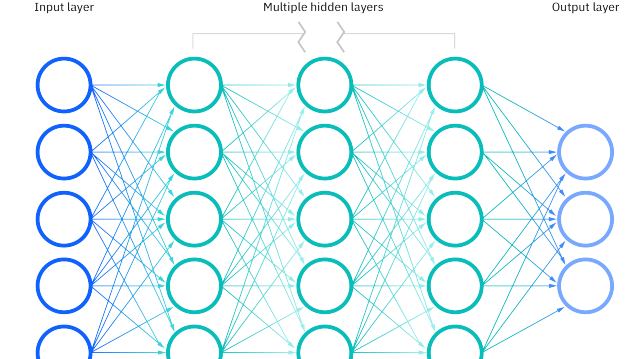
\includegraphics[width=\textwidth]{images/image012.png} \caption{Πλήρως διασυνδεμένο νευρωνικό δίκτυο [8]} 
% \label{fig:fc-network}
% \end{figure} 
\begin{Illustration}[!h] 
	\centering
	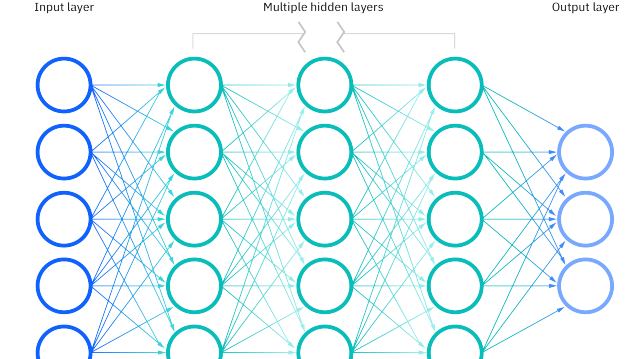
\includegraphics[width=0.6\textwidth]{images/image012.png} \caption{Πλήρως διασυνδεμένο νευρωνικό δίκτυο [8]} 
	\label{fc-network}
\end{Illustration}


Στο επίπεδο εισόδου τροφοδοτούμε τα δεδομένα τα οποία θα παράγουν μια έξοδο. Τα ενδιάμεσα επίπεδα ανάλογα με το είδος του επιπέδου εκτελούν υπολογισμούς και πράξεις στα δεδομένα. Προσθέτοντας επίπεδα αυξάνεται ο βαθμός ελευθερίας του νευρωνικού δικτύου και μπορεί να αναγνωρίσει πιο περίπλοκα μοτίβα και χαρακτηριστικά στα δεδομένα. Βαθιά νευρωνικά δίκτυα είναι αυτά που αποτελούνται από ένα μεγάλο αριθμό κρυφών επιπέδων. Το επίπεδο εξόδου συνήθως είναι ένας αριθμός που αντιπροσωπεύει τις βαθμολογίες των κλάσεων ταξινόμησης.

\subsection{Εκπαίδευση Νευρωνικών Δικτύων}

\subsubsection{Οπισθοδρομική Διάδοση - \en{Backpropagation}}

Κύριος στόχος της εκπαίδευσης ενός νευρωνικού δικτύου είναι η προσαρμογή των παραμέτρων του δικτύου ώστε να δίνουν όσο το δυνατόν πιο ακριβή αποτελέσματα για κάθε είσοδο. 

Αρχικά θέτονται τυχαίες τιμές στα βάρη του νευρωνικού και υπολογίζεται η έξοδος για μια είσοδο. Υπολογίζεται η διαφορά με την τιμή που θα περιμέναμε να έχει η έξοδος μέσο μιας συνάρτησης σφάλματος. Στόχος είναι η ελαχιστοποίηση του σφάλματος μεταβάλλοντας τα βάρη.

Η οπισθοδρομική διάδοση είναι η τεχνική που χρησιμοποιούμε για να βρούμε τα βέλτιστα βάρη, και αναφέρεται στη διάδοση αυτού του σφάλματος από την έξοδο στην είσοδο του δικτύου, υπολογίζοντας τις παραγώγους για την αναπροσαρμογή των παραμέτρων. Η διαδικασία αυτή γίνεται επαναληπτικά για πολλά δεδομένα έως ότου υπάρξει κάποια σύγκλιση.[9]

??Σε αυτή τη διπλωματική δεν θα ασχοληθούμε με το κομμάτι της εκπαίδευσης.

\subsection{Συνελικτικά Νευρωνικά Δίκτυα}

Τα συνελικτικά νευρωνικά δίκτυα \en{(Convolutional Neural Networks – CNN)}  είναι μια κατηγορία νευρωνικών δικτύων τα οποία χρησιμοποιούνται κυρίως στην υπολογιστική όραση καθώς έχουν πολύ καλή απόδοση σε δεδομένα που έχουν κάποια χωρική διάταξη, όπως οι εικόνες.

Τα συνελικτικά νευρωνικά δίκτυα είναι όμοια με τα πλήρως διασυνδεμένα νευρωνικά δίκτυα με τη διαφορά ότι αντί για νευρώνες έχουμε φίλτρα ή αλλιώς πυρήνες τα οποία εκτελούν τη μαθηματική πράξη της συνέλιξης. Τα φίλτρα είναι δισδιάστατοι πίνακες με εκπαιδεύσιμα βάρη με τα οποία σαρώνουμε τα δεδομένα εισόδου, δηλαδή τις εικόνες, για να εξάγουμε χαρακτηριστικά από αυτές. 

Εάν τροφοδοτήσουμε ένα πλήρως διασυνδεμένο νευρωνικό δίκτυο με μία εικόνα, κάθε πίξελ της εικόνας στην είσοδο συνδέεται με κάθε νευρώνα του κρυφού επιπέδου. Αρχικά, η δισδιάστατη εικόνα έχει μετατραπεί σε ένα μονοδιάστατο διάνυσμα με αποτέλεσμα να χάνεται κάθε χωρική πληροφορία που υπάρχει σε αυτή. Επιπλέον, για μία εικόνα $100\times100$ πίξελ, η οποία θεωρείται μικρή για τα σημερινά δεδομένα, χρειαζόμαστε 10.000 παραμέτρους για κάθε νευρώνα του κρυφού επιπέδου, πράγμα που αυξάνει πάρα πολύ τον αριθμό τον παραμέτρων του δικτύου.  Άρα, το πλήρως διασυνδεμένο νευρωνικό δίκτυο δεν αποτελεί καλό τρόπο επίλυσης του προβλήματος της αναγνώρισης εικόνων.

Χρησιμοποιώντας φίλτρα, κάθε νευρώνας βλέπει ένα μέρος της εικόνας και μας δίνει μία έξοδο που αντιστοιχεί σε αυτό το κομμάτι. Ολισθαίνοντας το φίλτρο σε όλη την εικόνα,  παίρνουμε σαν έξοδο μια άλλη εικόνα την οποία τροφοδοτούμε σε επόμενο επίπεδο. Με αυτό τον τρόπο έχουμε καταφέρει να διατηρήσουμε την χωρική πληροφορία που περιέχεται στην είσοδο μας και εκπαιδεύοντας τα βάρη στα φίλτρα, το δίκτυο μαθαίνει  να εντοπίζει χαρακτηριστικά και μοτίβα στις εικόνες. Επιπλέον, χρησιμοποιούμε τα ίδια βάρη για μια εικόνα, πράγμα  που μειώνει  το πλήθος των παραμέτρων του δικτύου.

Η πράξη της συνέλιξης μας δείχνει πόσο  κοντά είναι η εικόνα στο μοτίβο ή το χαρακτηριστικό στοιχείο που ψάχνουμε. Η εικόνα που παίρνουμε σαν αποτέλεσμα είναι μια απεικόνιση των χαρακτηριστικών \en{(feature map)}. Χρησιμοποιώντας πολλά φίλτρα μπορούμε να εξάγουμε διαφορετικά χαρακτηριστικά από την εικόνα. Με κάθε επίπεδο που προστίθεται το δίκτυο αυξάνει την πολυπλοκότητά του και αναγνωρίζει μεγαλύτερα τμήματα της εικόνας. Τα πρώτα επίπεδα επικεντρώνονται σε απλά χαρακτηριστικά, όπως χρώματα και ακμές. Καθώς η εικόνα επεξεργάζεται από τα διάφορα επίπεδα, το δίκτυο αρχίζει να αναγνωρίζει μεγαλύτερα στοιχεία της εικόνας ή σχήματα αντικειμένων έως ότου τελικά αναγνωρίσει το εικονιζόμενο αντικείμενο. [5], [8], [10], [11]
 
\begin{Illustration}[!ht] \centering
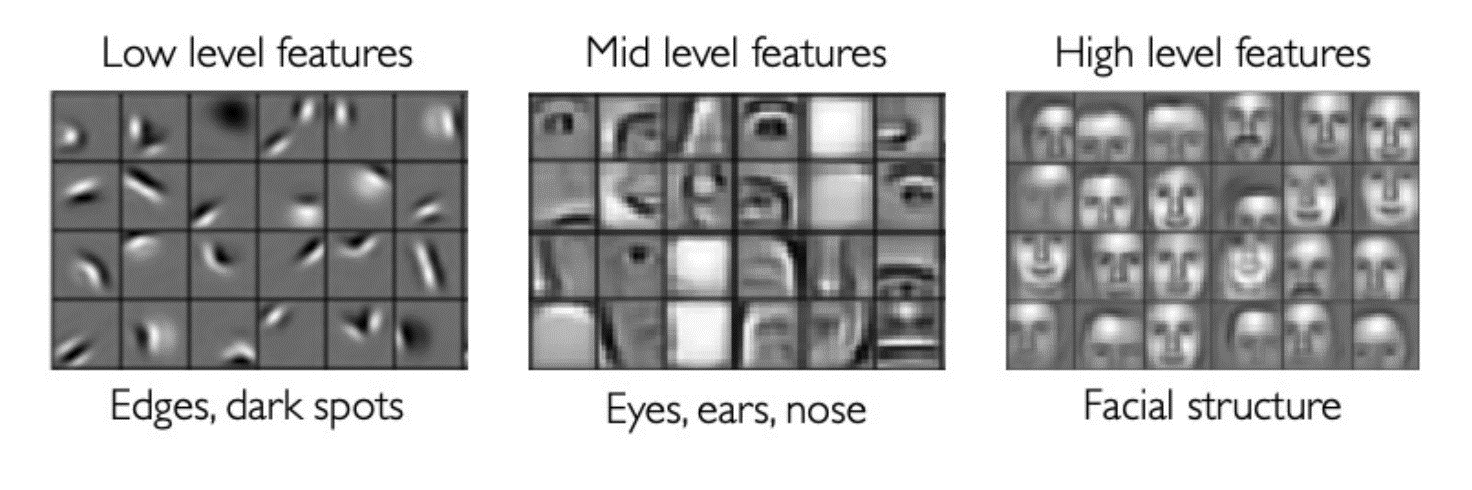
\includegraphics[width=\textwidth]{images/image014.png} \caption{Απεικόνιση χαρακτηριστικών που εξάγει το νευρωνικό δίκτυο στα επίπεδα  [10]} 
\label{fig:feature-exptraction}
\end{Illustration} 

\subsection{Επίπεδα Συνελικτικών Νευρωνικών Δικτύων}

Τα συνελικτικά νευρωνικά δίκτυα αποτελούνται από τρείς τύπους επιπέδων. Το συνελικτικό επίπεδο ακολουθούμενο από μια μη γραμμικότητα, το επίπεδο δειγματοληψίας και το πλήρως διασυνδεμένο επίπεδο. Μια απλή αρχιτεκτονική συνελικτικού δικτύου είναι η εξής:

\begin{enumerate}
    \item Το \textbf{επίπεδο εισόδου} είναι αυτό στο οποίο τροφοδοτούνται τα δεδομένα σε μορφή τρισδιάστατων πινάκων, για έγχρωμες εικόνες πλάτος, ύψος και τρία χρωματικά κανάλια \en{RGB}.
    \item \textbf{Συνελικτικό επίπεδο} \en{(convolution layer)} ακολουθούμενο από μία μη γραμμικότητα, συνήθως \en{ReLU}. Υπολογίζεται η συνέλιξη της εικόνας εισόδου με τα φίλτρα, και στη συνέχεια εφαρμόζεται η συνάρτηση ενεργοποίησης \en{ReLU} για κάθε στοιχείο της εξόδου.
    \item Tο \textbf{επίπεδο δειγματοληψίας} \en{(pooling layer)} είναι μία πράξη υποδειγματοληψίας που εφαρμόζουμε ώστε να μειώσουμε τη διάσταση των δεδομένων.
    \item Το \textbf{πλήρες διασυνδεμένο επίπεδο} \en{(fully connected layer)} είναι αυτό που κάνει την ταξινόμηση και μας δίνει την βαθμολογία της κάθε κλάσης.
\end{enumerate}

\begin{Illustration}[!ht] \centering
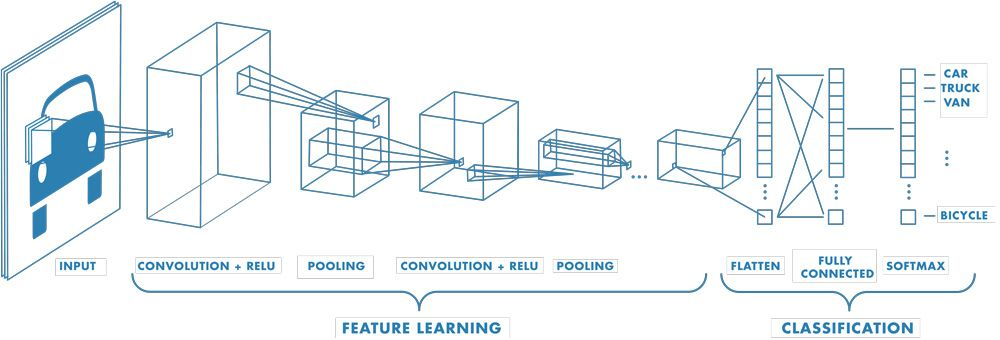
\includegraphics[width=\textwidth]{images/image015.jpg} \caption{Αρχιτεκτονκική συνελικτικού νευρωνικού δικτύου  [12]} 
\label{fig:}
\end{Illustration} 

	\chapter{Παράλληλος Προγραμματισμός}

Οι εφαρμογές σήμερα, έχουν όλο και μεγαλύτερες απαιτήσεις σε υπολογιστική ισχύ. Η εγκυρότητα των μετεωρολογικών προβλέψεων, η ακρίβεια των αναλύσεων των δομικών κατασκευών των μηχανικών, η δημιουργία ρεαλιστικών γραφικών στους υπολογιστές, ο αριθμός των αεροπορικών κρατήσεων που επεξεργάζονται ανά δευτερόλεπτο και ο αριθμός των μεταφορών κεφαλαίων που επεξεργάζονται ανά δευτερόλεπτο βασίζονται στην ταχύτητα επεξεργασίας μεγάλου όγκου δεδομένων. Επιπλέον, η πρόοδος που έχει σημειωθεί τα τελευταία χρόνια στον τομέα της τεχνητής νοημοσύνης, όπως η εξέλιξη στους αλγόριθμους μηχανικής μάθησης, οφείλεται στην μεγαλύτερη ταχύτητα εκτέλεσης και τους πόρους που προσφέρουν οι σύγχρονες υπολογιστικές συσκευές.

Τις δεκαετίες του 1980 και 1990, η ταχύτητα των μικροεπεξεργαστών άρχισε να αυξάνεται με μεγάλο ρυθμό, λόγο της αύξησης της ταχύτητας του ρολογιού της κεντρικής μονάδας επεξεργασίας και τις βελτιώσεις στο σχεδιασμό υλικών (\en{hardware}). Όμως, αυτή η τάση σταμάτησε το 2003, λόγω της μεγάλης κατανάλωσης ενέργειας που προκύπτει από την αύξηση της συχνότητας του ρολογιού και ζητήματα απαγωγής θερμότητας. Λύση σε αυτό το πρόβλημα δόθηκε με τη χρήση πολλαπλών επεξεργαστικών πυρήνων σε ένα υπολογιστικό σύστημα. Με αυτό τον τρόπο είναι δυνατή η εκτέλεση πολλών εντολών παράλληλα κρατώντας την κατανάλωση ενέργειας χαμηλά.

Για την αξιοποίηση της υπολογιστικής ισχύς των πολλαπλών πυρήνων, χρειάστηκε να γίνει αλλαγή στο προγραμματιστικό μοντέλο που ακολουθούσαμε μέχρι σήμερα. Παραδοσιακά, τα προγράμματα αποτελούνται από μια ακολουθία εντολών που εκτελούνται από έναν επεξεργαστή σειριακά. Ο παράλληλος προγραμματισμός αναφέρεται στον διαμοιρασμό μιας εργασίας σε επιμέρους διεργασίες οι οποίες μπορούν να εκτελεστούν ταυτόχρονα από διαφορετικές επεξεργαστικές μονάδες, με στόχο τη μείωση στο χρόνο εκτέλεσης.

Τα στοιχεία για παράλληλη επεξεργασία που συναντάμε σε κάθε υπολογιστή είναι η \en{CPU} – κεντρική μονάδα επεξεργασίας, και η \en{GPU} – κάρτα γραφικών. Η \en{CPU} εκτελεί όλους τους υπολογισμούς και διαχειρίζεται όλες τις διεργασίες που είναι απαραίτητες για τη λειτουργία ενός λειτουργικού συστήματος. Περιλαμβάνει ένα περίπλοκο σχεδιασμό ελέγχου που επιτρέπει μεγάλη ευελιξία και απόδοση. Η \en{GPU}, αν και αρχικά σχεδιάστηκε για να μπορεί να εκτελεί πολλές ταυτόχρονες πράξεις για γραφικά, περιλαμβάνει πολλά επεξεργαστικά στοιχεία με πιο απλό σχεδιασμό ελέγχου και πλέον χρησιμοποιείται και για προγραμματισμό γενικού σκοπού. Τα δύο αυτά στοιχεία συνεργάζονται για την πιο γρήγορη επίλυση προβλημάτων. Συνδέοντας πολλά μηχανήματα με επεξεργαστικά στοιχεία σε κόμβους ή μέσω δικτύων, μπορούμε να δημιουργήσουμε συστοιχίες υπολογιστών (\en{cluster}) με πολύ μεγάλη υπολογιστική ισχύ. [21]

\section{Παράλληλος προγραμματισμός με \en{CPU}}
Τα σύγχρονα υπολογιστικά συστήματα διαθέτουν επεξεργαστές \en{CPU} με πολλαπλούς πυρήνες και υλικό που προσφέρεται για παραλληλία. Υπάρχουν τρείς τρόποι που μια \en{CPU} επιτρέπει την επιτάχυνση μέσω παραλληλίας: χρήση διανυσματικών επεξεργαστών (\en{vectorization}), πολλαπλοί πυρήνες και νήματα (\en{threading}), διαμοιρασμένη μνήμη.

\subsubsection{Διανυσματικοί επεξεργαστές – \en{vector processors}}

Η σύγχρονη αρχιτεκτονική επεξεργαστών περιλαμβάνει χαρακτηριστικά όπως διευρυμένους καταχωρητές (\en{wide registers}) και διευρυμένες επεξεργαστικές μονάδες (\en{wide processing units}) που επιτρέπουν την επεξεργασία κατά διανύσματα (\en{vector processing}), δηλαδή ταυτόχρονη επεξεργασία των τιμών ενός διανύσματος αντί για μία τιμή. Αυτή η μέθοδος είναι γνωστή ως \en{SIMD – Single Instruction Multiple Data}, όπου μία εντολή χρησιμοποιείται για την επεξεργασία πολλών δεδομένων. Για παράδειγμα, για τον υπολογισμό του αθροίσματος δύο διανυσμάτων:

\selectlanguage{english}
\usemintedstyle{bw}

\begin{minted}{c}
    for (i = 0; i < count; i++) 
      c[i] = a[i] + b[i]; 
    }
\end{minted}
  \selectlanguage{greek}

% Εικόνα 3.1 
\begin{Illustration}[!h] 
	\centering
	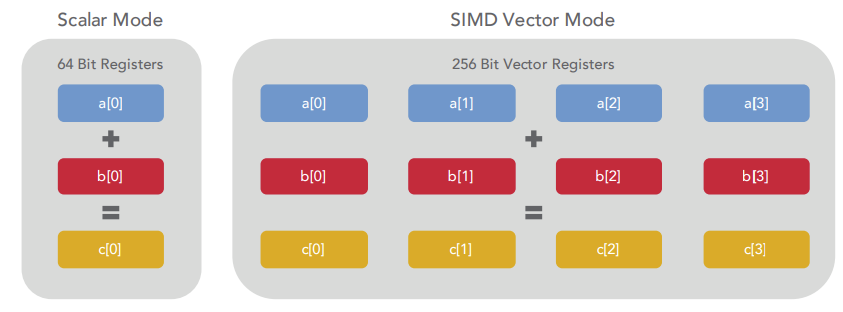
\includegraphics[width=\textwidth]{images/image043.png} 
	\caption{Πρόσθεση με χρήση διευρυμένους καταχωρητές 256\en{-bit} [22]}
	\label{image-registers-add}
\end{Illustration}

έστω ότι θέλουμε να υπολογίσουμε το άθροισμα αριθμών 64\en{-bit} διπλής ακρίβειας τύπου \src{float}. Αντί για το άθροισμα ενός ζεύγους αριθμών κάθε φορά, μπορούμε να χρησιμοποιήσουμε διευρυμένους καταχωρητές των 256\en{-bit} και να αθροίσουμε τέσσερα ζεύγη αριθμών ταυτόχρονα.
Ο πιο απλός τρόπος για την εφαρμογή της επεξεργασίας κατά διανύσματα είναι μέσω του μεταγλωττιστή (\en{compiler}) με την ενεργοποίηση των κατάλληλων επιλογών (\en{flags}). Στον \en{GCC compiler} προσθέτοντας τις επιλογές \src{-O3 ή -ftree-slp-vectorize, -ftree-vectorize,} μαζί με άλλες βελτιστοποιήσεις που πραγματοποιεί στον κώδικα, ο μεταγλωττιστής εντοπίζει τα τμήματα του κώδικα που θεωρεί ασφαλή για την εφαρμογή διανυσματικής επεξεργασίας. Με την επιλογή \src{-fopt-info-vec-optimized}, ο μεταγλωττιστής τυπώνει μηνύματα για τα τμήματα του κώδικα που έχουν υποστεί διανυσματική επεξεργασία. Αυτή η μέθοδος αποτελεί έναν γρήγορο και απλό τρόπο για βελτιστοποίηση της . Ωστόσο, ο μεταγλωττιστής δεν μπορεί πάντα να αναγνωρίσει όλα τα τμήματα του κώδικα που μπορούν να βελτιστοποιηθούν, καθώς μπορεί να χρειάζεται περισσότερες πληροφορίες.

Μπορούμε να δώσουμε περισσότερες πληροφορίες στον μεταγλωττιστή για τη δομή του κώδικα και να έχουμε καλύτερο έλεγχο της διανυσματοποίησης (\en{vectorization}) με εντολές τύπου \src{pragma}. Οι εντολές αυτές είναι για τον προεπεξεργαστή (\en{preprocessor}) και ξεκινάνε με τη δήλωση \src{\#pragma}. Τέτοιες εντολές παρέχει η \en{OpenMP}, στην οποία θα αναφερθούμε εκτενέστερα παρακάτω. Ένα απλό παράδειγμα φαίνεται εδώ:

\selectlanguage{english}
\begin{minted}{c}
    #pragma omp simd
    for (int n = 0; n < N; n++)
      a[n] += b[n];
\end{minted}
\selectlanguage{greek}

Οι εντολές τύπου \src{\#pragma} έχουν καλύτερη απόδοση σε σύγκριση με την απλή προσθήκη επιλογών βελτιστοποίησης (\en{flags}) στον μεταγλωττιστή, καθώς επιτρέπουν την εφαρμογή διανυσματικής επεξεργασίας ακόμα και σε περιπτώσεις περίπλοκων βρόχων.
Για ακόμη μεγαλύτερο έλεγχο στις \en{SIMD} πράξεις χρησιμοποιούμε εσωτερικές συναρτήσεις \en{(intrinsics) SSE (Streaming SIMD Extensions} – Επεκτάσεις \en{SIMD} συνεχούς ροής) και \en{AVX (Advanced Vector Extensions} – Προχωρημένες επεκτάσεις διανυσμάτων), τα οποία είναι δύο σύνολα εντολών που αναγνωρίζει ο μεταγλωττιστής και επιτρέπει τον ορισμό πράξεων σε χαμηλότερο επίπεδο.

Ένα παράδειγμα για το πώς φαίνεται ο κώδικας για πολλαπλασιασμό πίνακα με διάνυσμα υλοποιημένος με εσωτερικές συναρτήσεις φαίνεται παρακάτω:
 
\subsubsection{Πολλαπλοί πυρήνες και νήματα}

Οι σύγχρονοι επεξεργαστές διαθέτουν πάνω από έναν πυρήνα και κοινή μνήμη στην οποία όλοι οι πυρήνες έχουν πρόσβαση. Οι πολλαπλοί πυρήνες επιτρέπουν την εκτέλεση διεργασιών ταυτόχρονα ώστε να μειώνεται ο συνολικός χρόνος εκτέλεσης ενός προγράμματος. Το νήμα (\en{thread}), είναι μία ακολουθία εκτέλεσης εντολών μέσα σε μία διεργασία. Όλα τα νήματα που ανήκουν στην ίδια διεργασία έχουν πρόσβαση στα δεδομένα της διεργασίας σε κοινή μνήμη αλλά μπορούν να εκτελούνται παράλληλα.
 
% Εικόνα 3.2 
\begin{Illustration}[!h] 
	\centering
	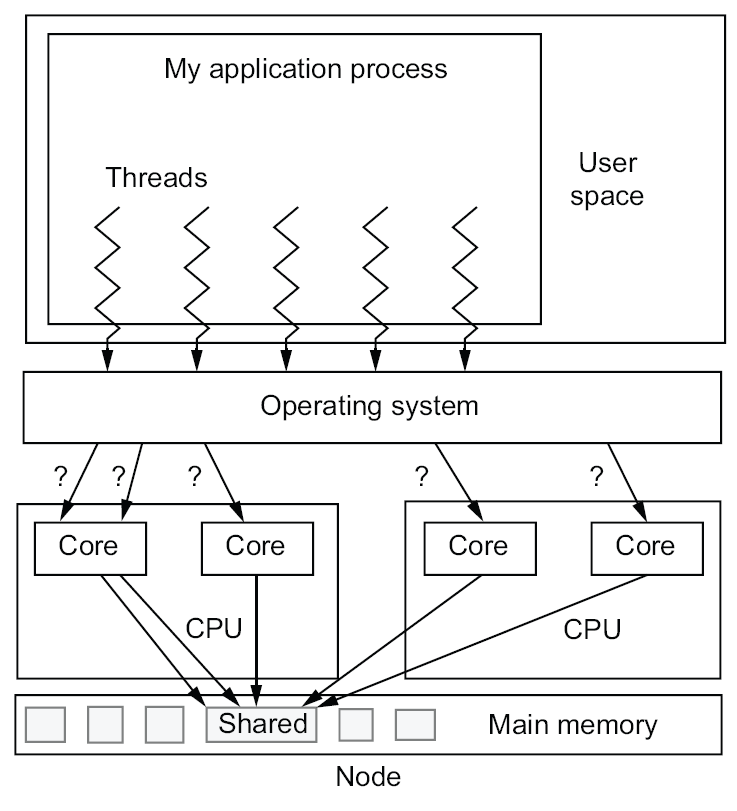
\includegraphics[width=0.45\textwidth]{images/image045.png} 
	\caption{Σύστημα πολλαπλών πυρήνων και κοινής μνήμης [23]}
	\label{image-multicore-shared-mem}
\end{Illustration}

\subsection{\en{OpenMP}}

To \en{OpenMP} χρησιμοποιείται για ανάπτυξη πολυνηματικών (\en{multithreaded}) παράλληλων εφαρμογών σε συστήματα κοινής μνήμης. Είναι ένα \en{API (Application Programming Interface} – Διεπαφή προγραμματισμού εφαρμογής) που επιτρέπει την εύκολη επεκτασιμότητα σειριακών προγραμμάτων γραμμένων σε \en{C,C++} ή \en{Fortran} σε παράλληλα με τη χρήση οδηγιών (\en{directives}) προς τον μεταγλωττιστή και μιας βιβλιοθήκης συναρτήσεων. Οι οδηγίες ορίζουν στο σειριακό πρόγραμμα περιοχές του κώδικα που μπορούν να εκτελεστούν παράλληλα και δίνουν πληροφορίες στον μεταγλωττιστή σχετικά με τις μεταβλητές και τον τρόπο διαμοιρασμού των επαναλήψεων ενός βρόχου στα διαθέσιμα νήματα. Δίνει έναν εύκολο και ευέλικτο τρόπο βελτιστοποίησης της ταχύτητας με παράλληλο προγραμματισμό. 
Ένα παράδειγμα κώδικα φαίνεται παρακάτω:

\selectlanguage{english}
\begin{minted}{text}
    #pragma omp parallel for
    for (int i = 0;i < N; i++)
        do_work(i);
\end{minted}

\selectlanguage{greek}

Οι οδηγίες του \en{OpenMP} ξεκινάνε με \src{\#pragma omp} και με το \src{parallel} δημιουργεί νήματα καθένα από τα οποία θα εκτελέσουν ένα αντίγραφο του κώδικα που βρίσκεται μέσα στο δομημένο μπλοκ. Με το for οι επαναλήψεις μοιράζονται μεταξύ των νημάτων. Στο τέλος του μπλοκ, τα νήματα συγχρονίζονται και αφού όλα τελειώσουν του υπολογισμούς τους, το πρόγραμμα συνεχίζει την εκτέλεση του. Στην περίπτωση που ο μεταγλωττιστής ή το μηχάνημα που διαθέτουμε δεν υποστηρίζει παραλληλία με \en{OpenMP}, αγνοούνται οι εντολές \src{\#pragma} και το πρόγραμμα τρέχει κανονικά με σειριακό τρόπο.

Το \en{OpenMP} διαθέτει πολλά στοιχεία για δημιουργία νημάτων, διαμοιρασμό της εργασίας, διαχείριση του περιβάλλοντος μεταβλητών και λειτουργίες συγχρονισμού των νημάτων. Τα τελευταία χρόνια έχουν προστεθεί και λειτουργίες για υποστήριξη παραλληλίας σε κάρτες γραφικών.

\subsection{Προγραμματισμός σε \en{GPU}}

Τα τελευταία χρόνια, οι κάρτες γραφικών χρησιμοποιούνται για προγραμματισμό γενικής χρήσης. Αρχικά, οι \en{GPU} σχεδιάστηκαν με σκοπό την επιτάχυνση υπολογισμών που έχουν να κάνουν με γραφικά. Γι’ αυτό το λόγο, διαθέτουν πολλούς απλούς επεξεργαστές που μπορούν να εκτελούν μαζικά αριθμητικές πράξεις. Σήμερα, οι προγραμματιστές εκμεταλλεύονται την αρχιτεκτονική των \en{GPU} για την επιτάχυνση επιστημονικών και άλλων εφαρμογών. 
Η διαφορά με τις \en{CPU} είναι πως οι \en{GPU} εστιάζουν στην διεκπεραιωτική ικανότητα εκτέλεσης (\en{throughput}) των παράλληλων εφαρμογών, ενώ οι \en{CPU} εστιάζουν στην γρήγορη ταχύτητα εκτέλεσης (\en{latency}) σειριακών προγραμμάτων. Σε σχέση με την \en{CPU}, η \en{GPU} διαθέτει πολλούς επεξεργαστές, απλούς, λιγότερο ισχυρούς και με πιο χαλαρό μοντέλο μνήμης ώστε περισσότερα δεδομένα να επεξεργάζονται ταυτόχρονα. Αυτό έχει και σαν αποτέλεσμα την χαμηλότερη κατανάλωση ενέργειας σε σχέση με τις \en{CPU} αλλά λιγότερο ευέλικτες προγραμματιστικά. 
 
% Εικόνα 3.3 
\begin{Illustration}[!h] 
	\centering
	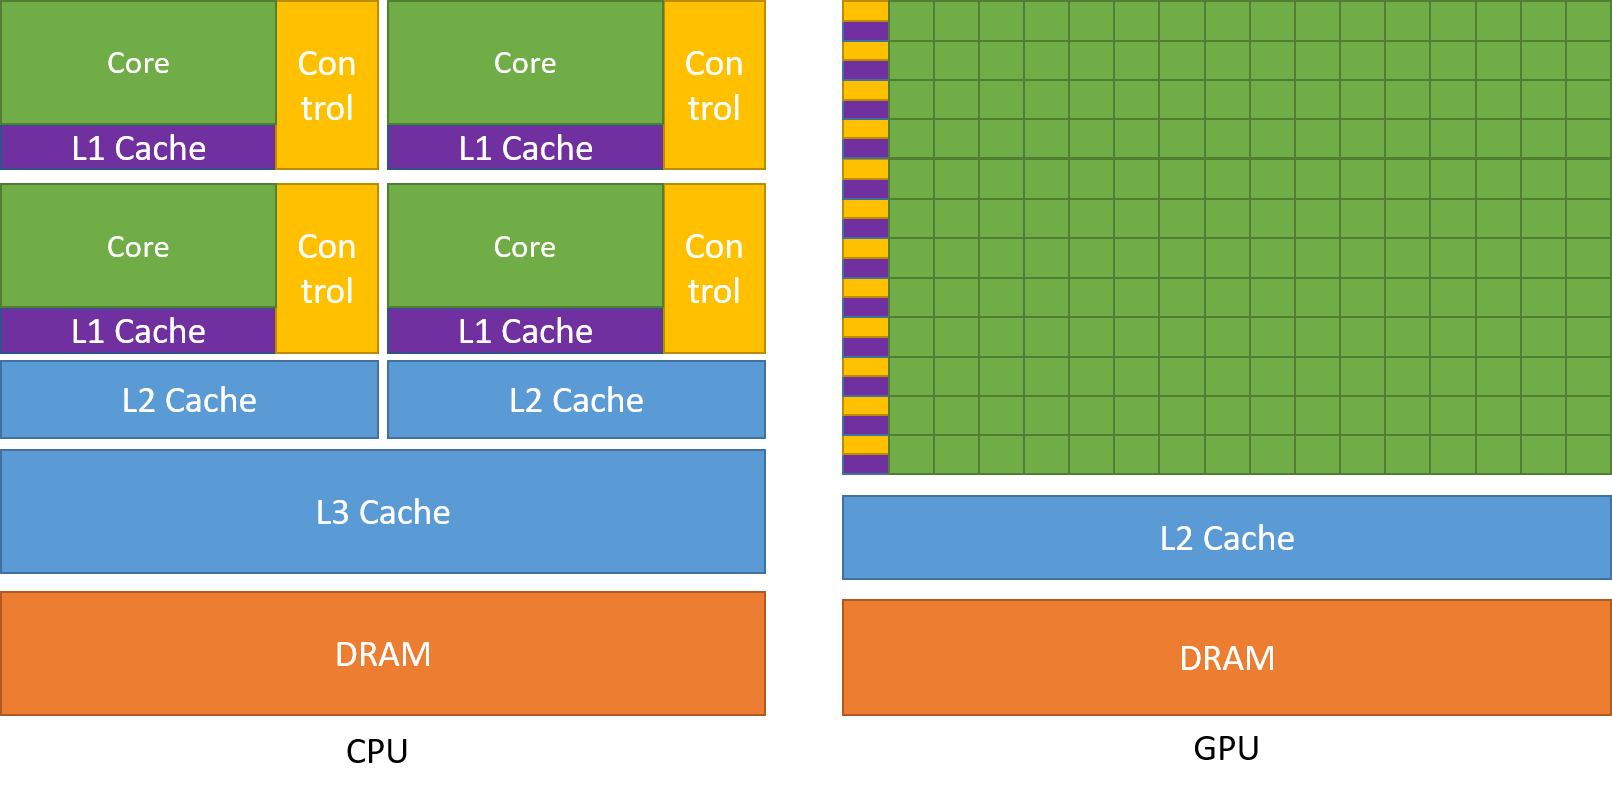
\includegraphics[width=0.8\textwidth]{images/image046.png} 
	\caption{Διαφορές αρχιτεκτονικής \en{CPU} και \en{GPU} [24]}
	\label{image-3.3}
\end{Illustration}

\subsection{\en{CUDA}}
Η \en{CUDA} είναι μια πλατφόρμα για παράλληλο προγραμματισμό και ένα προγραμματιστικό μοντέλο που αναπτύχθηκε από την \en{NVIDIA} για προγραμματισμό γενικού σκοπού σε κάρτες γραφικών \en{(GPGPU – General-Purpose Graphics Processing Unit).} Υποστηρίζει προγραμματισμό στις γλώσσες \en{C,C++, Fortran, Python} και \en{MATLAB} με επεκτάσεις σε αυτές για παράλληλο προγραμματισμό σε \en{GPU} της εταιρίας.

\subsection{Προγραμματιστικό Μοντέλο}

% Εικόνα 3.4 
\begin{Illustration}[!h] 
	\centering
	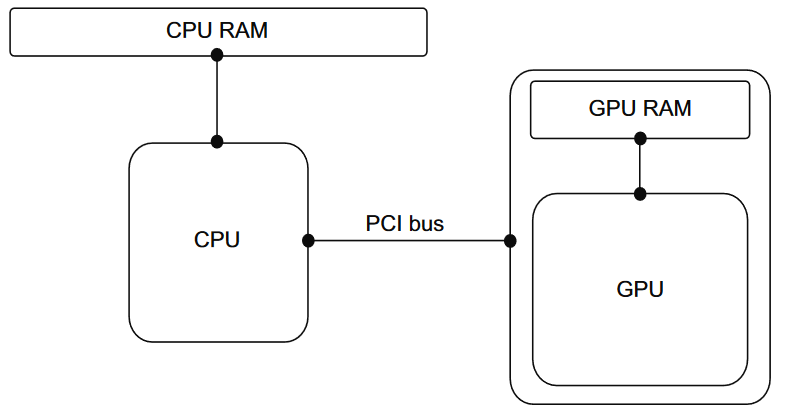
\includegraphics[width=0.75\textwidth]{images/image047.png} 
	\caption{Ετερογενές Σύστημα με \en{GPU} [23]}
	\label{image-3.4}
\end{Illustration}

Το προγραμματιστικό μοντέλο της \en{CUDA} αναφέρεται σε συστήματα ετερογενή, δηλαδή συστήματα που διαθέτουν δύο διαφορετικούς επεξεργαστές σε αυτά, την \en{CPU} και την \en{GPU}. Η \en{CPU} στην οποία τρέχει το κυρίως πρόγραμμα ονομάζεται κεντρικό σύστημα - \en{host} και η \en{GPU}, η οποία λειτουργεί βοηθητικά και θα εκτελέσει το υπολογιστικά βαρύ μέρος του κώδικα, ονομάζεται συσκευή - \en{device}. Η \en{GPU} λειτουργεί σαν συνεπεξεργαστής στο κεντρικό σύστημα, την \en{CPU}. Επίσης, η \en{CPU} και η \en{GPU} έχει η κάθε μία τη δική της ξεχωριστή μνήμη. 

Η \en{CPU} τρέχει το κυρίως πρόγραμμα και στέλνει εντολές στην \en{GPU} για το τι να κάνει. Είναι υπεύθυνη για την μεταφορά δεδομένων από και προς την \en{GPU}, την δέσμευση μνήμης στην \en{GPU} και την εκκίνηση συναρτήσεων που θα εκτελεστούν στην \en{GPU}.

Τα κομμάτια του κώδικα που θα εκτελεστούν στη συσκευή, στο κυρίως πρόγραμμα εμφανίζονται με τη μορφή συναρτήσεων και ονομάζονται πυρήνες (\en{kernels}). Όταν καλείται μια συνάρτηση πυρήνα, η συσκευή εκκινεί έναν μεγάλο αριθμό νημάτων που θα εκτελέσουν τον πυρήνα. Όλα τα νήματα που παράγει ένας πυρήνας σε μία κλήση συνολικά ονομάζονται πλέγμα (\en{grid}). Όταν ολοκληρωθεί η εκτέλεση όλων των νημάτων που ανήκουν στο ίδιο πλέγμα, η εκτέλεση του προγράμματος συνεχίζει στο κεντρικό σύστημα, μέχρι να συναντήσει τον επόμενο πυρήνα. [21]
 
% Εικόνα 3.5 
\begin{Illustration}[!h] 
	\centering
	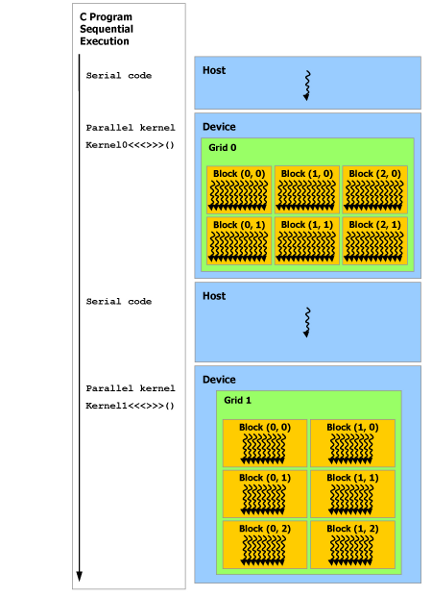
\includegraphics[width=0.5\textwidth]{images/image048.png} 
	\caption{Ροή εκτέλεσης προγράμματος σε ετερογενές σύστημα με \en{GPU} [24]}
	\label{image-3.5}
\end{Illustration}

Τα νήματα που ανήκουν σε ένα πλέγμα οργανώνονται σε μπλοκ (\en{block}). Όλα τα μπλοκ ενός πλέγματος έχουν τον ίδιο αριθμό νημάτων. Ο μέγιστος αριθμός νημάτων που μπορεί να έχει ένα μπλοκ εξαρτάται από την αρχιτεκτονική της κάρτας γραφικών, συνήθως είναι 1024.
 
% Εικόνα 3.6 
\begin{Illustration}[!h] 
	\centering
	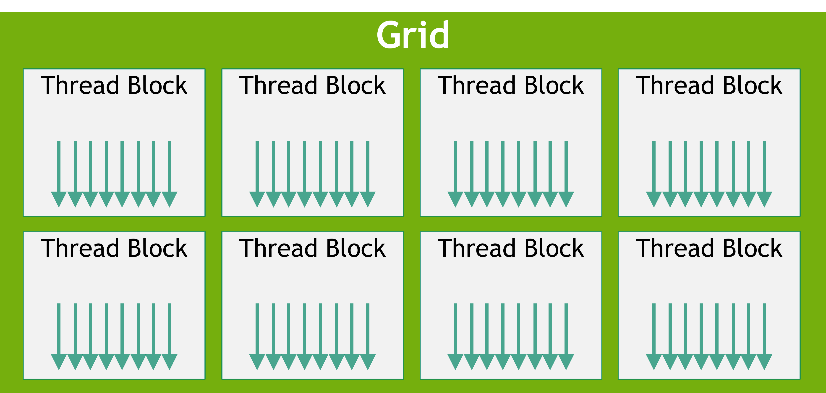
\includegraphics[width=0.7\textwidth]{images/image049.png} 
	\caption{Ένα πλέγμα από μπλοκ νημάτων [24]}
	\label{image-3.6}
\end{Illustration}

\subsubsection{Αρχιτεκτονική Κάρτας Γραφικών}
 
% Εικόνα 3.7 
\begin{Illustration}[!h] 
	\centering
	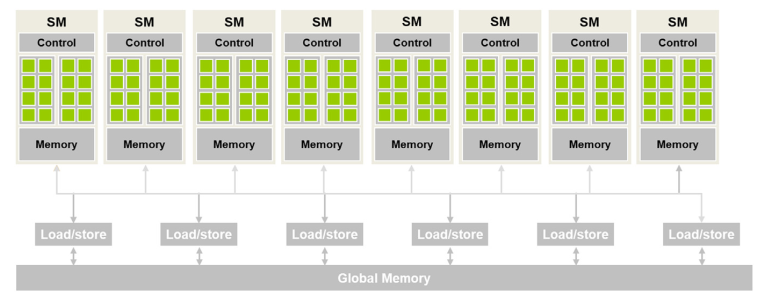
\includegraphics[width=\textwidth]{images/image050.png} 
	\caption{Αρχιτεκτονική Κάρτας Γραφικών [21]}
	\label{image-3.7}
\end{Illustration}


Αυτή η οργάνωση των νημάτων σε μπλοκ και πλέγματα προκύπτει από την αρχιτεκτονική της \en{GPU}. H \en{GPU} αποτελείται από πολυεπεξεργαστές συνεχούς ροής - \en{SM (streaming multiprocessors)} και κάθε \en{SM} διαθέτει πολλούς μικρούς επεξεργαστές που μπορούν να τρέχουν νήματα παράλληλα.

Όταν το σύστημα καλεί μια συνάρτηση πυρήνα εκκινείτε ένα πλέγμα από νήματα που θα εκτελέσουν τον κώδικα του πυρήνα. Η \en{GPU} αναλαμβάνει τον τρόπο διαμοιρασμού των μπλοκ νημάτων. Κάθε μπλοκ ανατίθεται σε ένα \en{SM}, ώστε τα νήματα που ανήκουν σε αυτό να εκτελεστούν παράλληλα. Η ανάθεση ενός μπλοκ σε ένα \en{SM} επιτρέπει στα νήματα που ανήκουν σε αυτό να αλληλεπιδρούν μεταξύ τους. Πολλά μπλοκ μπορούν να ανατεθούν στο ίδιο \en{SM}, όμως υπάρχει ένα όριο στο πόσα μπορούν να εκτελεστούν ταυτόχρονα.

Η \en{CUDA} δεν μπορεί να εγγυηθεί για τη σειρά και σε ποιο \en{SM} θα εκτελεστεί το κάθε μπλοκ. Αυτό δίνει το πλεονέκτημα στην \en{GPU} να είναι ευέλικτη και αποδοτική στην οργάνωση της εκτέλεσης των εργασιών. Επιπλέον, η εκτέλεση ενός προγράμματος \en{CUDA} είναι ανεξάρτητη του αριθμού των \en{SM} της συσκευής, πράγμα που σημαίνει πως το ίδιο πρόγραμμα μπορεί να τρέξει σε μια απλή συσκευή με ένα \en{SM}, αλλά και σε υπερυπολογιστή που διαθέτει πολλές \en{GPU}.

Όμως, δεν υπάρχει τρόπος να γνωρίζουμε σε ποιο \en{SM} θα εκτελεστεί το κάθε μπλοκ και δεν υπάρχει άμεσος τρόπος επικοινωνίας μεταξύ των μπλοκ. Εάν ένα μπλοκ περιμένει ένα άλλο για να ολοκληρωθεί, μπορεί να οδηγηθούμε σε αδιέξοδο (\en{dead lock}) εάν το δεύτερο μπλοκ έχει ολοκληρωθεί. Όλα τα νήματα που ανήκουν στο ίδιο μπλοκ πρέπει να ολοκληρωθούν ώστε να προγραμματιστεί η εκτέλεση του επόμενου μπλοκ στο \en{SM}.

\subsubsection{Μνήμη Κάρτας Γραφικών}
 
% Εικόνα 3.8 
\begin{Illustration}[!h] 
	\centering
	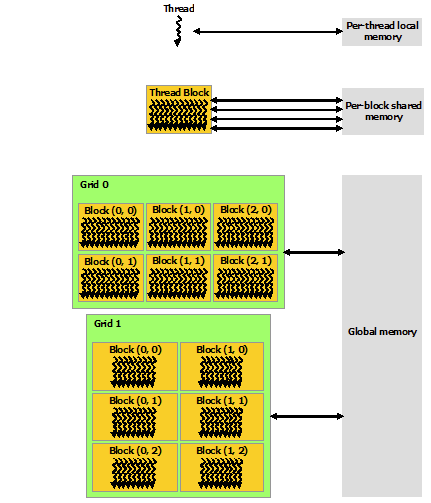
\includegraphics[width=0.65\textwidth]{images/image051.png} 
	\caption{Ιεραρχία μνήμης κάρτας γραφικών \en{CUDA} [24]}
	\label{image-3.8}
\end{Illustration}

Οι κάρτες γραφικών διαθέτουν τη δική τους μνήμη με δική της ιεραρχία. Κάθε νήμα έχει τοπική μνήμη (\en{local memory}), ιδιωτική για το νήμα. Κάθε μπλοκ από νήματα διαθέτει μια κοινή μνήμη (\en{shared memory}) στην οποία έχουν πρόσβαση όλα τα νήματα που ανήκουν σε αυτό. Είναι μνήμη που ανήκει στον \en{SM} και επιτρέπει την συνεργασία των νημάτων που ανήκουν στο ίδιο μπλοκ. Τέλος, υπάρχει και η καθολική μνήμη (\en{global memory}), από την οποία μπορούν να διαβάζουν και να γράφουν όλα τα νήματα οποιαδήποτε στιγμή. 

Η καθολική μνήμη είναι ο κύριος χώρος αποθήκευσης της κάρτας γραφικών και χρησιμοποιείται για την μεταφορά δεδομένων μεταξύ της \en{CPU} και της \en{GPU}. Ο προγραμματιστής χρειάζεται να δεσμεύσει χώρο στην καθολική μνήμη της συσκευής και να μεταφέρει δεδομένα από την μνήμη του κεντρικού συστήματος στην καθολική μνήμη της συσκευής. Μετά την εκτέλεση τον υπολογισμών στην συσκευή ο προγραμματιστής χρειάζεται να μεταφέρει τα αποτελέσματα πίσω στη μνήμη του κεντρικού συστήματος και να αποδεσμεύσει την μνήμη που δεν χρειάζεται πια από τη συσκευή. 

\subsubsection{Συγχρονισμός}

Τα νήματα έχουν πρόσβαση στα αποτελέσματα άλλων νημάτων μέσω της κοινής και της καθολικής μνήμης. Μπορούν να εργαστούν μαζί σε έναν υπολογισμό, αλλά με κάποιους περιορισμούς. Καθώς η \en{CUDA} δεν μπορεί να εγγυηθεί για την σειρά με την οποία θα εκτελεστούν τα νήματα, υπάρχει ο κίνδυνος ένα νήμα να διαβάσει ένα αποτέλεσμα πριν ένα άλλο νήμα υπολογίσει και γράψει το αποτέλεσμα αυτό.
 
% Εικόνα 3.9 
\begin{Illustration}[!h] 
	\centering
	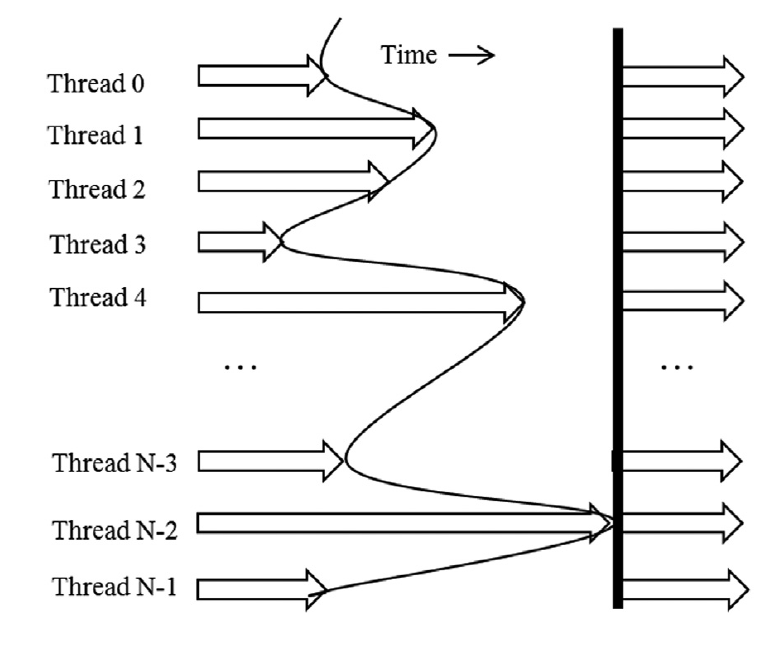
\includegraphics[width=0.5\textwidth]{images/image052.png} 
	\caption{Παράδειγμα συγχρονισμού των \en{threads} σε \en{barrier} [21]}
	\label{image-3.9}
\end{Illustration}


Η \en{CUDA} διαθέτει συναρτήσεις για συγχρονισμό των νημάτων. Ο πιο απλός τρόπος συγχρονισμού είναι το φράγμα (\en{barrier}). Το φράγμα είναι ένα σημείο στο πρόγραμμα όπου όλα τα νήματα σταματάνε και περιμένουν. Όταν όλα τα νήματα έχουν φτάσει στο φράγμα, μπορούν να συνεχίσουν την εκτέλεση του υπόλοιπου κώδικα.

\subsubsection{Πρόγραμμα σε \en{CUDA}}
Ένα τυπικό πρόγραμμα σε \en{CUDA} αποτελείται από την εξής ακολουθία εντολών:
\begin{enumerate}
\item Δήλωση μεταβλητών και δέσμευση μνήμης στο κεντρικό σύστημα και την συσκευή.
\item Αρχικοποίηση των δεδομένων στο κεντρικό σύστημα
\item Μεταφορά των δεδομένων από το κεντρικό σύστημα στη συσκευή
\item Εκτέλεση ενός ή περισσότερων πυρήνων
\item Μεταφορά των αποτελεσμάτων από την συσκευή στο κεντρικό σύστημα
\end{enumerate}

Ένα απλό πρόγραμμα \en{CUDA} που εκτελεί πρόσθεση δύο διανυσμάτων παράλληλα φαίνεται παρακάτω:
 
% Εικόνα 3.10
\begin{Illustration}[!h] 
	\centering
	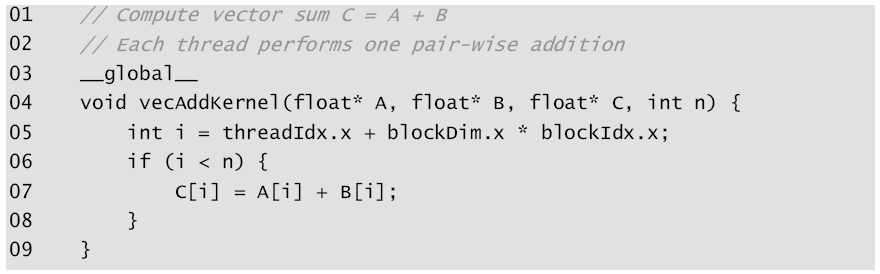
\includegraphics[width=0.6\textwidth]{images/image053.png} 
	\caption{Κώδικας συνάρτησης πυρήνα – \en{CUDA} [21]}
	\label{image-3.10}
\end{Illustration}


Με το \src{\_\_global\_\_} δηλώνεται η συνάρτηση πυρήνα που θα εκτελεστεί στη συσκευή.
Με την συνάρτηση \src{CUDAMalloc()} γίνεται η δέσμευση μνήμης στη συσκευή και στη συνέχεια με την \src{CUDAMemcpy()} αντιγράφονται οι τιμές των μεταβλητών. Η κλήση της συνάρτησης πυρήνα ακολουθείται από τα σύμβολα \mbox{\src{\en{< < <...> > >}}} με τα οποία δηλώνονται o αριθμός των νημάτων ανά μπλοκ και των μπλοκ στο πλέγμα που θα εκκινηθούν από τη συσκευή. Αφού εκτελεστεί ο πυρήνας, αντιγράφουμε τα αποτελέσματα από την συσκευή στο κεντρικό σύστημα με την \src{CUDAMemcpy()} και τέλος αποδεσμεύουμε την μνήμη της συσκευής για κάθε μεταβλητή με την \src{CUDAFree()}. 
 
% Εικόνα 3.11 
\begin{Illustration}[!h] 
	\centering
	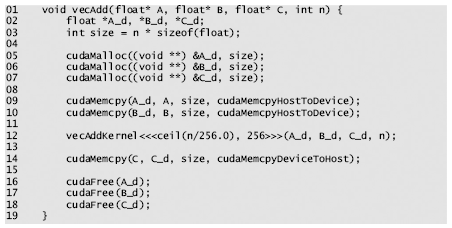
\includegraphics[width=0.6\textwidth]{images/image054.png} 
	\caption{Πάράδειγμα κώδικα σε \en{CUDA} [21]}
	\label{image-3.11}
\end{Illustration}

\subsection{\en{OpenCL}}

Μια άλλη επιλογή για παράλληλο προγραμματισμό ετερογενών συστημάτων είναι η \en{OpenCL}. Είναι ένα ανοικτό, δωρεάν πρότυπο για παράλληλο προγραμματισμό που υποστηρίζει κάρτες γραφικών όπως \en{NVIDIA} και \en{AMD} και σε πολλές άλλες συσκευές υλικού (\en{hardware}). Επιπλέον, είναι συμβατή με τους περισσότερους μεταγλωττιστές για \en{C} και \en{C++}. 

Η \en{OpenCL} είναι ένα αρκετά χαμηλού επιπέδου προγραμματιστικό μοντέλο με ευρεία αποδοχή, αλλά μακροσκελή (\en{verbose}) σύνταξη. Ένας από τους λόγους για τους οποίους η \en{OpenCL} θεωρείται ότι είναι μακροσκελής είναι ότι η επιλογή της συσκευής είναι αρκετά περίπλοκη. Ο προγραμματιστής πρέπει να εντοπίσει και να επιλέξει τη συσκευή στην οποία θα εκτελεστεί κάποια διεργασία και αυτό μπορεί να ανέλθει σε εκατοντάδες γραμμές κώδικα μόνο για να ξεκινήσει. 

Όπως και στην \en{CUDA} , έτσι και στην \en{OpenCL} ένα πρόγραμμα αποτελείται από δύο μέρη, τους πυρήνες που εκτελούνται στην συσκευή και το πρόγραμμα του κεντρικού συστήματος (\en{host}) που διαχειρίζεται την εκτέλεση των πυρήνων. Παρακάτω φαίνεται η αντιστοιχία της ορολογίας που χρησιμοποιεί η \en{OpenCL} με αυτή της \en{CUDA}.


\begin{table}[!h]
    \centering
    \selectlanguage{english}
    \begin{tabular}{ll}
        \textbf{OpenCL} & \textbf{CUDA} \\
        \hline
        NDRange & Grid \\
        Work Item & Thread \\
        Work Group & Block \\
        \hline
        Global Memory & Global Memory \\
        Local Memory & Shared Memory \\
        Private Memory & Local Memory \\
        Compute Unit & Streaming Multiproocessor \\
        Processing Element & Compute Core \\
        Work Item & Thread \\
        \hline
    \end{tabular}
    \selectlanguage{greek}
    \caption{Αντιστοιχεία \en{OpenCL} και \en{CUDA}}
    \label{tab:opencl-cuda}
\end{table}


Όπως αναφέρθηκε, η \en{OpenCL} μπορεί να υποστηρίξει πολλές διαφορετικές συσκευές υλικού, γι’ αυτό το λόγο έχει σύνθετο μοντέλο διαχείρισης των συσκευών. Η διαχείριση των συσκευών γίνεται με τον ορισμό του πλαισίου (\en{context}). Το πλαίσιο στην \en{OpenCL} είναι ο χώρος που περιλαμβάνει τις συσκευές, τη μνήμη για κάθε συσκευή και μια ουρά εντολών (\en{command queue}) ανά συσκευή. H ουρά εντολών είναι ο τρόπος που αλληλοεπιδρά το κεντρικό σύστημα με τις συσκευές για εκτέλεση πυρήνων, μεταφορές δεδομένων και λειτουργίες συγχρονισμού.
 
% Εικόνα 3.12 
\begin{Illustration}[!h] 
	\centering
	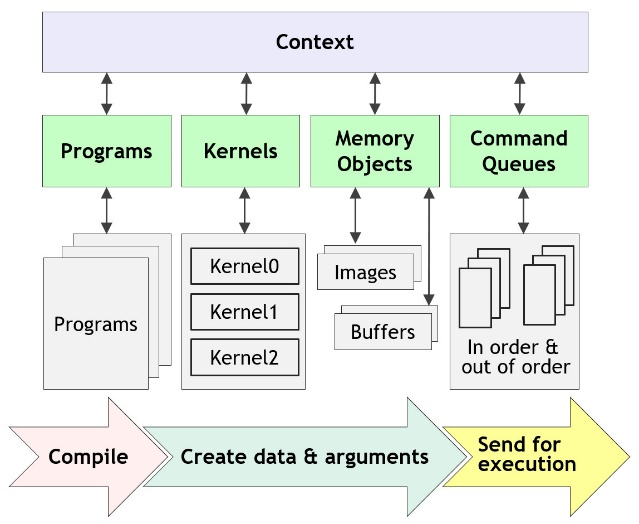
\includegraphics[width=0.5\textwidth]{images/image055.jpg} 
	\caption{Ακολουθία για εκτέλεση των πυρήνων στην \en{OpenCL} [25]}
	\label{image-3.12}
\end{Illustration}

Η \en{CUDA} εκτελεί αντίστοιχες διαδικασίες με την \en{OpenCL}, αλλά κρύβει την πολυπλοκότητα παρέχοντας τη δική της διεπαφή (\en{API}) για χρήση με συμβατές κάρτες γραφικών. 

\subsection{\en{OpenACC}}

Η \en{OpenACC} είναι ένα προγραμματιστικό μοντέλο, υψηλού επιπέδου, που βασίζεται σε οδηγίες προς τον μεταγλωττιστή (\en{directives}), σχεδιασμένο για \en{C/C++} και \en{Fortran} που δίνει λύση στην χρήση των \en{GPU} για επιτάχυνση υπολογισμών. Παρέχει μια απλοποιημένη προσέγγιση για τον προγραμματισμό ετερογενών αρχιτεκτονικών για υπολογιστική υψηλών επιδόσεων \en{(High-Performance Computing - HPC)}, επιτρέποντας στους προγραμματιστές να εισάγουν υποδείξεις στον κώδικά τους σχετικά με τον τρόπο που μπορεί να παραλληλοποιηθεί.

Το μοντέλο της \en{OpenACC} επιτρέπει στους επιστήμονες και τους προγραμματιστές να επικεντρωθούν στο επιστημονικό τους έργο χωρίς να χρειάζεται σε βάθος γνώση της αρχιτεκτονικής του υλικού (\en{hardware}), όπως για παράδειγμα στην \en{CUDA}. Οι προγραμματιστές μπορούν απλώς να εισάγουν οδηγίες στον κώδικά τους και ο μεταγλωττιστής αναλαμβάνει την παραλληλοποίηση και βελτιστοποίηση του κώδικα για την πλατφόρμα που έχει επιλεχθεί.

Το πλεονέκτημα του προγραμματισμού με οδηγίες είναι πως ο μεταγλωττιστής μπορεί να αγνοήσει τις οδηγίες και ο κώδικας να τρέξει σειριακά παράγοντας σωστά αποτελέσματα. Αυτό επιτρέπει τη διατήρηση μιας ενιαίας βάσης κώδικα, και επιπλέον, προσφέρει φορητότητα σε διαφορετικές πλατφόρμες. Η \en{OpenACC} χρησιμοποιείται κυρίως για παράλληλο προγραμματισμό σε κάρτες γραφικών, αλλά υποστηρίζει και άλλες αρχιτεκτονικές πολυπύρηνων επεξεργαστών. Μέχρι σήμερα, οι πλατφόρμες που υποστηρίζουν \en{OpenACC} περιλαμβάνουν τις αρχιτεκτονικές \en{x86} και \en{x64}, τις κάρτες γραφικών της \en{NVIDIA} και της \en{AMD}, επεξεργαστές \en{OpenPOWER, Knights Landing} και \en{ARM}. [26]

\subsubsection{Σύνταξη \en{OpenACC}}

Το \en{OpenACC} αποτελείται ένα σύνολο οδηγιών (\en{directives}) προς τον μεταγλωττιστή, βιβλιοθήκης συναρτήσεων και μεταβλητών περιβάλλοντος που επιτρέπει στον προγραμματιστή να εκφράσει τον παραλληλισμό που ενυπάρχει στον κώδικά, ώστε ο μεταγλωττιστής να μπορεί να τον μεταφράσει σε μορφή που να ταιριάζει σε διάφορες παράλληλες αρχιτεκτονικές.

Η σύνταξη των \textit{οδηγιών} προς τον μεταγλωττιστή σε \en{C/C++} έχει την παρακάτω μορφή:

\medskip
\src{\#pragma acc <directive> [clause [[,] clause] . . .] new-line}
\medskip

Η εντολές προς τον μεταγλωττιστή ξεκινούν με \src{\#pragma}, όπως ακριβώς και στην \en{OpenMP}. Το \src{acc} δηλώνει ότι αναφερόμαστε στην \en{OpenACC} και ακολουθείται από κάποιο \src{directive} το οποίο δίνει οδηγίες στον μεταγλωττιστή για το μπλοκ κώδικα που ακολουθεί. Το \en{clause} που είναι \textit{φράσεις} που παραμετροποιούν τη λειτουργία των \textit{οδηγιών}. 

Όπως σε κάθε γλώσσα προγραμματισμού για \en{GPU}, έτσι και στην \en{OpenACC}, υπάρχουν διάφορα στοιχεία που πρέπει να υπάρχουν και να εκτελούν τις εξής λειτουργίες:

\begin{enumerate}
\item Έκφραση των υπολογιστικών βρόχων σε παράλληλη μορφή για την \en{GPU}.
\item Μετακίνηση δεδομένων μεταξύ του κεντρικού συστήματος και της συσκευής
\item Λειτουργίες συγχρονισμού των νημάτων.
\end{enumerate}

Αυτά στην \en{OpenACC} υλοποιούνται με τις \textit{οδηγίες} που διαθέτει.

\subsubsection{Παραλληλοποίηση Κώδικα}

Το πιο βασικό στην \en{OpenACC} είναι ο διαμοιρασμός της εργασίας στα παράλληλα νήματα ώστε να επιτευχθεί καλύτερη απόδοση και να μειωθεί ο χρόνος εκτέλεσης. Η \en{OpenACC} διαμοιράζει τους βρόχους των επαναλήψεων σε νήματα αναθέτοντας μία επανάληψη ανά νήμα. Οι \textit{οδηγίες} που το κάνουν αυτό είναι το \src{kernels} και το \src{parallel}. 

Η \textit{οδηγία} \src{kernels}, δίνει εντολή στον μεταγλωττιστή να εντοπίσει τους βρόχους που μπορούν να εκτελεστούν παράλληλα στον κώδικα που βρίσκεται στο μπλοκ. Ο προγραμματιστής αφήνει τον μεταγλωττιστή να αναλύσει τον κώδικα και να παραλληλίσει τους βρόχους που θεωρεί πως είναι ασφαλές να το κάνει. Εάν θεωρήσει πως δεν μπορεί να παραλληλοποιηθεί, ο κώδικας θα τρέξει σειριακά. Και στις δύο περιπτώσεις ο μεταγλωττιστής εξασφαλίζει τα σωστά αποτελέσματα.

\selectlanguage{english}
\begin{minted}{c}
    #pragma acc kernels
    {
        for (int i = 0; i < N; i++) {
          c[i] = a[i] + b[i];
        }
        for (int i = 0; i < N; i++) {
          d[i] = a[i] + 5;
        }
    }
\end{minted}
\selectlanguage{greek}

Με την \textit{οδηγία} \src{parallel}, ο προγραμματιστής ενημερώνει τον μεταγλωττιστή ότι ο κώδικας μπορεί να παραλληλιστεί. Ο μεταγλωττιστής δημιουργεί \textit{ομάδες εργασίας} (\en{gangs}) στη συσκευή και κάθε ομάδα εργασίας θα εκτελέσει ολόκληρο το βρόχο που ακολουθεί. Οι \textit{ομάδες εργασίας}, είναι ομάδες από νήματα που ανήκουν σε \textit{μονάδες εργασίας} (\en{worker threads}) που εκτελούνται ανεξάρτητα, τα οποία αναλύονται παρακάτω. Για να διαμοιραστούν οι επαναλήψεις του βρόχου σε νήματα που θα εκτελεστούν παράλληλα, χρειάζεται η \textit{οδηγία} \src{loop}. 
 
% Εικόνα 3.13 
\begin{Illustration}[!h] 
	\centering
	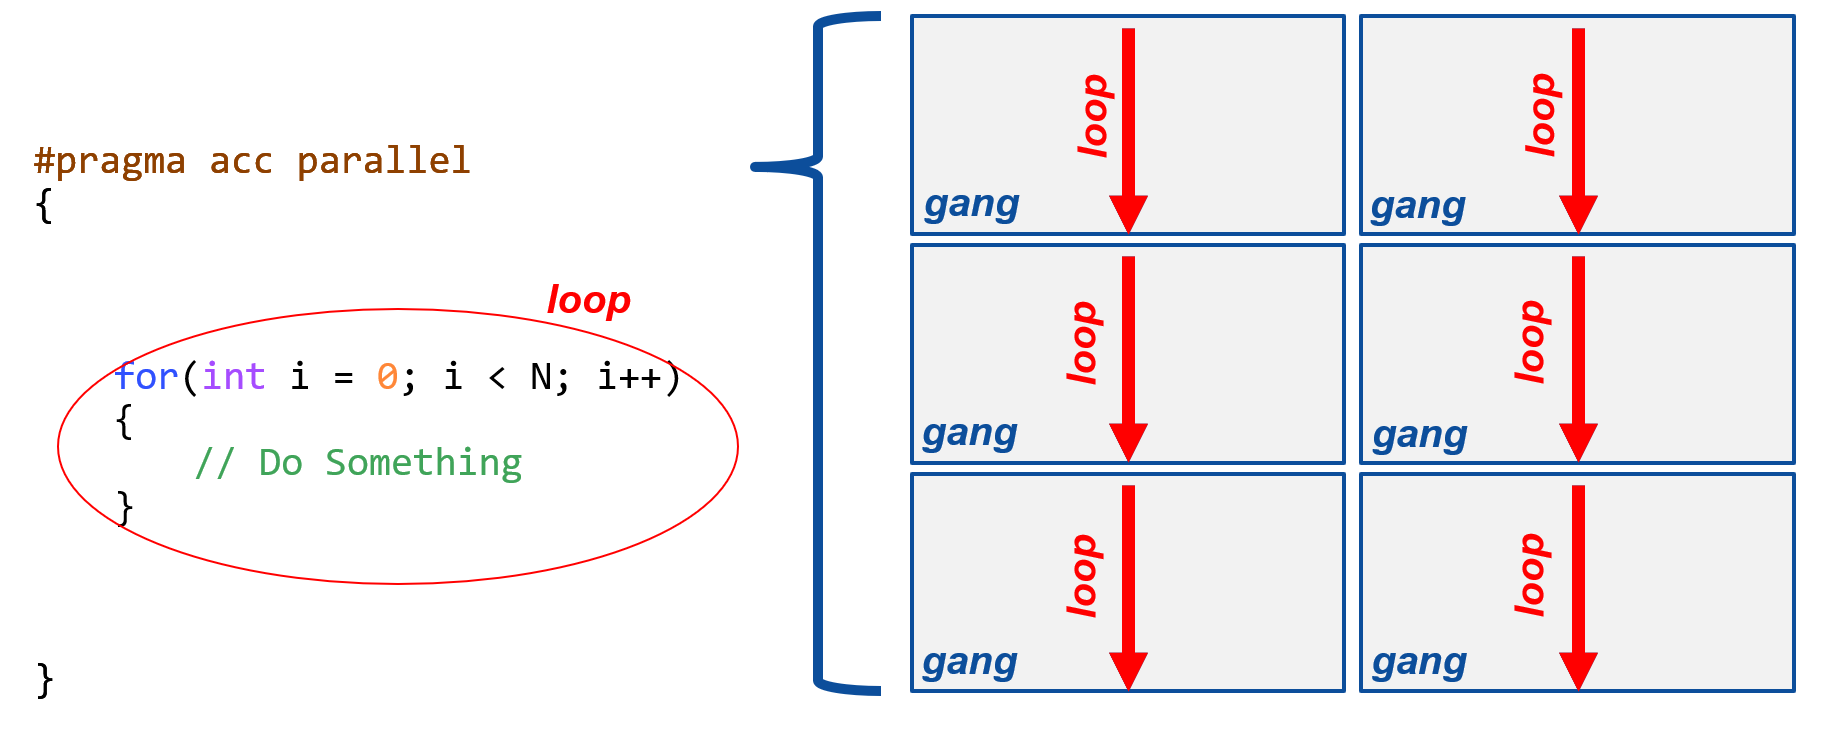
\includegraphics[width=0.7\textwidth]{images/image056.png} 
	\caption{ο βρόχος (\en{loop}) εκτελείται από όλες της ομάδες εργασίας (\en{gang}) [27]}
	\label{image-3.13}
\end{Illustration}

 
% Εικόνα 3.14 
\begin{Illustration}[!h] 
	\centering
	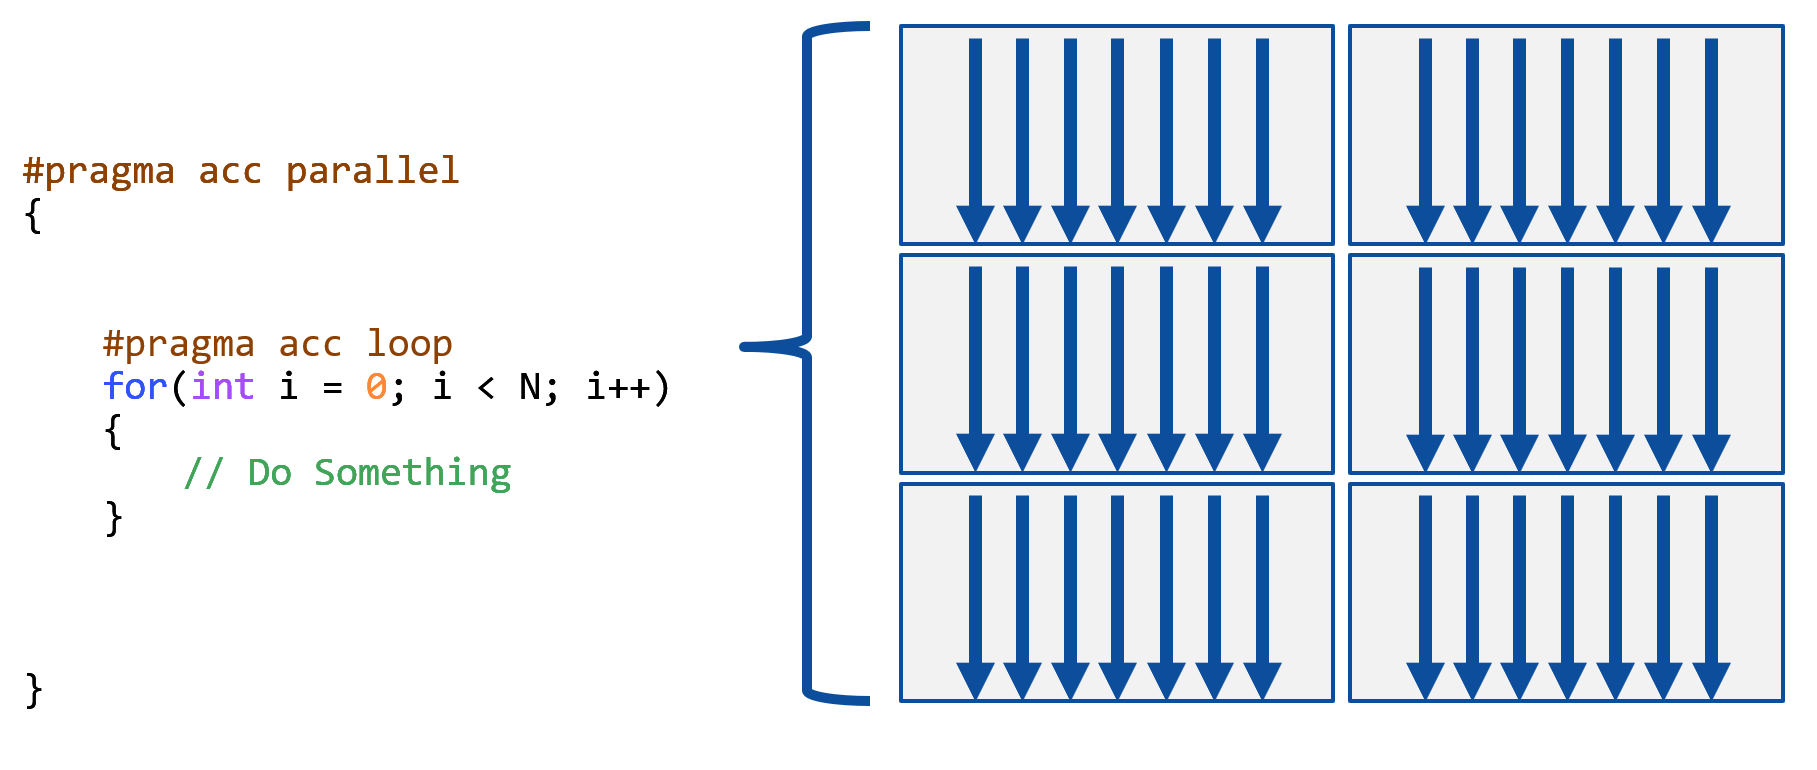
\includegraphics[width=0.7\textwidth]{images/image057.png} 
	\caption{με τη χρήση του \src{loop} οι επαναλήψεις διαμοιράζονται στις ομάδες εργασίας (\en{gang}) [27]}
	\label{image-3.14}
\end{Illustration}


Οι δύο \textit{οδηγίες} χρησιμοποιούνται συνδυαστικά και αναφέρονται στο βρόχο που ακολουθεί την εντολή \src{\#pragma}. Καθώς τον έλεγχο για την παραλληλοποίηση του κώδικα την έχει ο προγραμματιστής, θέλει προσοχή καθώς πιθανές εξαρτήσεις μεταξύ των δεδομένων στις επαναλήψεις μπορεί να οδηγήσουν σε λάθος αποτελέσματα.
  
\selectlanguage{english}
\begin{minted}{c}
    #pragma acc parallel loop
        for (int i = 0; i < N; i++) {
          c[i] = a[i] + b[i];
        }
    #pragma acc parallel loop
        for (int i = 0; i < N; i++) {
          d[i] = a[i] + 5;
        }
\end{minted}
\selectlanguage{greek}

Επιπλέον, το \src{loop} μπορεί να χρησιμοποιηθεί μέσα σε περιοχή που ορίζεται από την \textit{οδηγία} \src{kernels} σε περιπτώσεις που ο μεταγλωττιστής δεν μπορεί να αποφασίσει εάν είναι ανεξάρτητες οι επαναλήψεις μεταξύ τους.

\bigskip
\textbf{\textit{Υποβίβαση - \en{Reduction}}}
\medskip

Μία ειδική κατηγορία αλγορίθμων την οποία ο μεταγλωττιστής συνήθως δεν θα μπορέσει να παραλληλοποιήσει, είναι όταν μια μεταβλητή ή ένας πίνακας ενημερώνεται κατά τη διάρκεια κάθε επανάληψης ενός βρόχου. Ένα παράδειγμα τέτοιων αλγορίθμων είναι η εύρεση μέγιστου ή ελάχιστου ή ο υπολογισμός συνολικού αθροίσματος. Στον παράλληλο προγραμματισμό, οι πράξεις αυτές ονομάζονται \textit{πράξεις υποβίβασης} (\en{reduction}). Στην πράξη, αυτό που γίνεται είναι ότι ορίζεται μία μεταβλητή όπου το κάθε νήμα κάνει υπολογισμούς τοπικά, και στη συνέχεια ακολουθεί μία τελική πράξη που θα συνδυάσει όλες τις τοπικές μεταβλητές σε μία. 

Στην \en{OpenACC}, αυτό υλοποιείται με την \textit{φράση} \en{reduction} και χρησιμοποιείται ως εξής: 

\selectlanguage{english}
\begin{minted}{c}
        total = 0;
    #pragma acc parallel loop reduction(+ : total)
        for (i = 0; i < 100; i++) {
            total = total + data[i];
        }
\end{minted}
\selectlanguage{greek}

\subsubsection{Περιβάλλον Μεταβλητών}
 
% Εικόνα 3.15 
\begin{Illustration}[!h] 
	\centering
	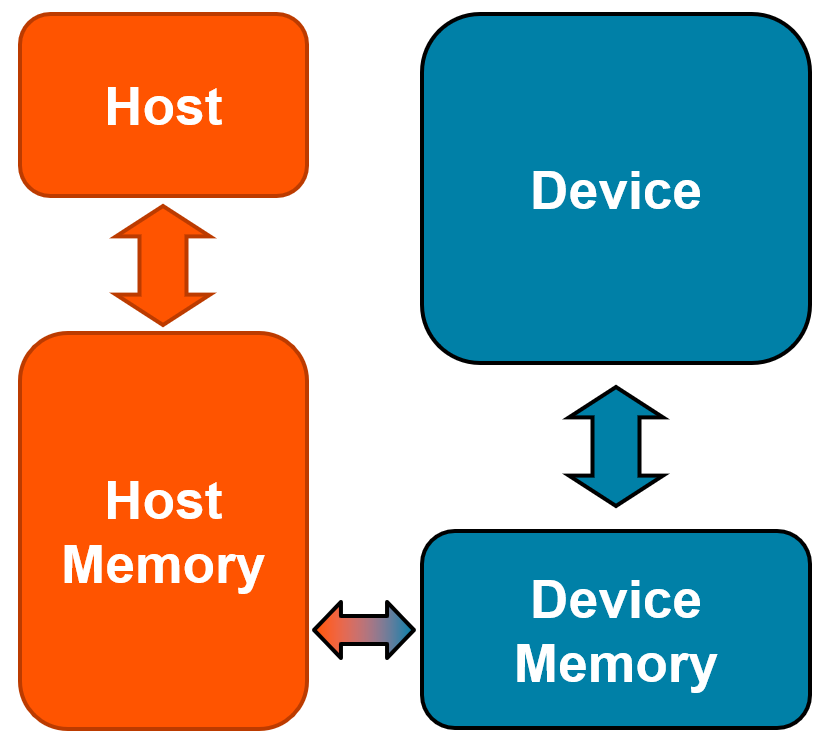
\includegraphics[width=0.5\textwidth]{images/image058.png} 
	\caption{Μοντέλο ετερογενούς συστήματος κεντρικού συστήματος (\en{host}) – συσκευής (\en{device}) [27]}
	\label{image-3.15}
\end{Illustration}


H \en{OpenACC} είναι σχεδιασμένη για ετερογενή συστήματα στα οποία η μνήμη της συσκευής που χρησιμοποιείται για την επιτάχυνση είναι ξεχωριστή από τη μνήμη του κεντρικού συστήματος, όπου τρέχει το κυρίως πρόγραμμα. Γι’ αυτό το λόγο είναι απαραίτητη η μεταφορά δεδομένων μεταξύ του κεντρικού συστήματος και της συσκευής. Στο μοντέλο της \en{OpenACC}, οι μεταφορές των δεδομένων γίνονται αυτόματα από τον μεταγλωττιστή, σε αντίθεση με τις γλώσσες χαμηλού επιπέδου, όπως η \en{CUDA}, όπου οι εντολές για δέσμευση μνήμης και μεταφοράς δεδομένων καταλαμβάνουν μεγάλο μέρος του κώδικα. 

Ωστόσο, ο μεταγλωττιστής για να εξασφαλίσει την σωστή λειτουργία του κώδικα, μπορεί να πραγματοποιεί περιττές μεταφορές δεδομένων από και προς τη μνήμη. Ο προγραμματιστής εισάγοντας τις κατάλληλες οδηγίες δίνει τις κατάλληλες πληροφορίες. Η εισαγωγή \textit{οδηγιών} για μεταφορά δεδομένων θεωρείται βελτιστοποίηση και πραγματοποιείται αφού έχουμε παραλληλοποιήσει τον κώδικα. 

Μερικές χαρακτηριστικές λειτουργίες που μπορεί να υποστηρίξει η \en{OpenACC} με χρήση \textit{φράσεων} (\en{clauses}) είναι: 

\begin{itemize}
\item \src{copy} – δεσμεύει μνήμη στη συσκευή για τις σχετικές μεταβλητές, αντιγράφει το περιεχομένων των μεταβλητών στη συσκευή, και αντιγράφει τα αποτελέσματα στο κεντρικό σύστημα στο τέλος της περιοχής.
\item \src{copyin} – έχει την ίδια λειτουργία με το \src{copy} με τη διαφορά πως στο τέλος της περιοχής δεν αντιγράφει το περιεχόμενο των μεταβλητών στο κεντρικό σύστημα.
\item \src{copyout} – ίδια λειτουργία με το \src{copy} με τη διαφορά πως δημιουργεί τις μεταβλητές χωρίς να τις αρχικοποιήσει, αντιγράφει μόνο τα αποτελέσματα στο τέλος από τη συσκευή στο κεντρικό σύστημα.
\item \src{create} – δεσμεύει χώρο στη συσκευή για τις σχετικές μεταβλητές, και απελευθερώνει τον χώρο στο τέλος της περιοχής, αλλά δεν αντιγράφει δεδομένα από και προς τη συσκευή.
\item \src{present} – δηλώνει πως οι μεταβλητές υπάρχουν στην συσκευή και δεν χρειάζεται γίνει κάποια ενέργεια. [28]
\end{itemize}

Η χρήση των παραπάνω \textit{φράσεων} συνδυάζεται με της \textit{οδηγίες} \src{parallel} και \src{kernels} που ορίζουν περιοχές παραλληλίας, αλλά και με την \textit{οδηγία} \src{data}, με το οποίο ο χρήστης ορίζει \textit{περιοχές δεδομένων} (\en{data regions}) που ορίζουν την \textit{διάρκεια ζωής των δεδομένων} (\en{data lifetime}) στην συσκευή.

\selectlanguage{english}
   \begin{minted}{c}
    #pragma acc data create(x[0:N]) copyout(y[0:N])
    {
    #pragma acc parallel loop
    for (i = 0; i < N; i++) {
      y[i] = 0.0f;
      x[i] = (float)(i + 1);
    }
    
    #pragma acc parallel loop
    for (i = 0; i < N; i++) {
      y[i] = 2.0f * x[i] + y[i];
    }
    }
\end{minted}
  \selectlanguage{greek}


\subsection{Επίπεδα παραλληλισμού}

Για να εξασφαλίσει τη φορητότητα σε διαφορετικές αρχιτεκτονικές, η \en{OpenACC} ορίζει ένα αφαιρετικό μοντέλο για την απεικόνιση των πολλαπλών επιπέδων παραλληλισμού που μπορεί να διαθέτει ένας επεξεργαστής. Διακρίνονται τρία επίπεδα παραλληλίας: \textit{ομάδα εργασίας} - \en{gang}, \textit{μονάδα εργασίας} ή \textit{εργάτης} - \en{worker} και \textit{διάνυσμα} - \en{vector}. 
 
% Εικόνα 3.16 
\begin{Illustration}[!h] 
	\centering
	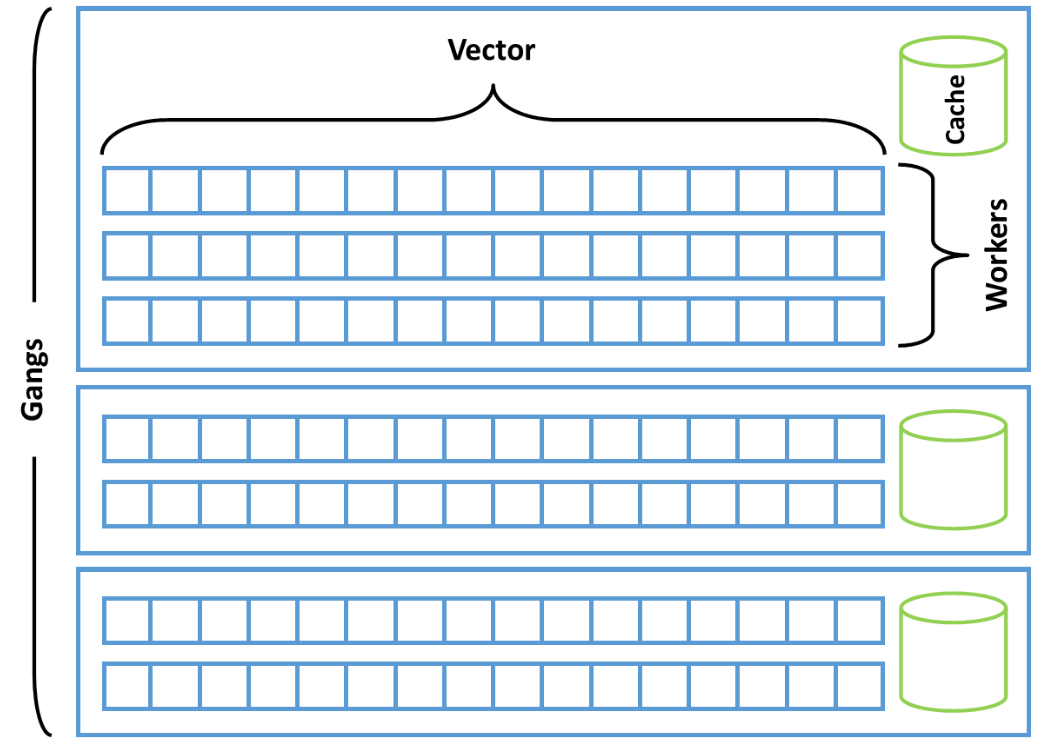
\includegraphics[width=0.6\textwidth]{images/image059.png} 
	\caption{Επίπεδα παραλληλισμού της \en{OpenACC} [28]}
	\label{image-3.16}
\end{Illustration}


Το \textit{διάνυσμα} (\en{vector}) είναι το χαμηλότερο επίπεδο παραλληλίας και αναφέρεται στην εκτέλεση της ίδιας εντολής σε διαφορετικά δεδομένα – \en{SIMD (Single instruction, Multiple Data} – μια εντολή, πολλά δεδομένα) για τις \en{CPU} ή \en{SIMT (Single Instruction, Multiple Threads} – μία εντολή, πολλά νήματα) στις \en{GPU}. Το μήκος του διανύσματος – \en{vector length} δηλώνει σε πόσα στοιχεία δεδομένων θα εκτελεστεί η ίδια εντολή. Η \textit{ομάδα εργασίας} (\en{gang}) είναι το υψηλότερο επίπεδο παραλληλίας, όπου κάθε \textit{ομάδα} εκτελείται ανεξάρτητα από τις άλλες και δε συγχρονίζονται μεταξύ τους. Η \textit{μονάδα εργασίας }ή\textit{ εργάτης} (\en{worker}) είναι ανάμεσα στα δύο επίπεδα. Μία \textit{ομάδα εργασίας} αποτελείται από έναν ή περισσότερους \textit{εργάτες}, οι οποίοι λειτουργούν σε ένα διάνυσμα κάποιου μήκους. Οι \textit{εργάτες} και τα διάνυσμα που ανήκουν στην ίδια \textit{ομάδα} έχουν πρόσβαση σε μία κοινή κρυφή μνήμη (\en{cache}) και επιτρέπεται ο συγχρονισμός μεταξύ τους.[28]

Για βελτιστοποίηση στον τρόπο αντιστοίχισης στο διαθέσιμο υλικό, η \en{OpenACC} διαθέτει φράσεις (\en{clauses}) για διαμοιρασμό της εργασίας. Μερικά ενδεικτικά είναι\src{ seq, auto, gang, worker, vector, tile, num\_gangs, num\_workers,} και \src{vector\_length}. [26]

    \part{Πρακτικό Μέρος} 
	\chapter{Ανάλυση και σχεδίαση}
\InitialCharacter{Σ}το κεφάλαιο αυτό παρουσιάζεται η μελέτη που έγινε για την υλοποίηση του συστήματος. Αρχικά περιγράφεται η αρχιτεκτονική του
συστήματος και γίνεται ο διαχωρισμός του στα επιμέρους
υποσυστήματα, ενώ στη συνέχεια περιγράφονται οι εφαρμογές του
συστήματος.

\section{Ανάλυση - περιγραφή αρχιτεκτονικής}
Στην ενότητα αυτή παρουσιάζεται η ανάλυση του συστήματος και ο
χωρισμός του σε υποσυστήματα όσον αφορά την αρχιτεκτονική.

\subsection{Διαχωρισμός υποσυστημάτων}
Το σύστημα αποτελείται από τους απλούς κόμβους και ένα κόμβο
διαχειριστή. Στο σημείο αυτό αναλύουμε το σύστημα ενός απλού
κόμβου, το οποίο αποτελείται από τα εξής υποσυστήματα:

\begin{itemize}
\item Υποσύστημα δημιουργίας σχήματος.
\item Υποσύστημα ενσωμάτωσης δεδομένων στο σχήμα.
\item Υποσύστημα επικοινωνίας κόμβου.
\end{itemize}

\begin{figure}[!ht] \centering
	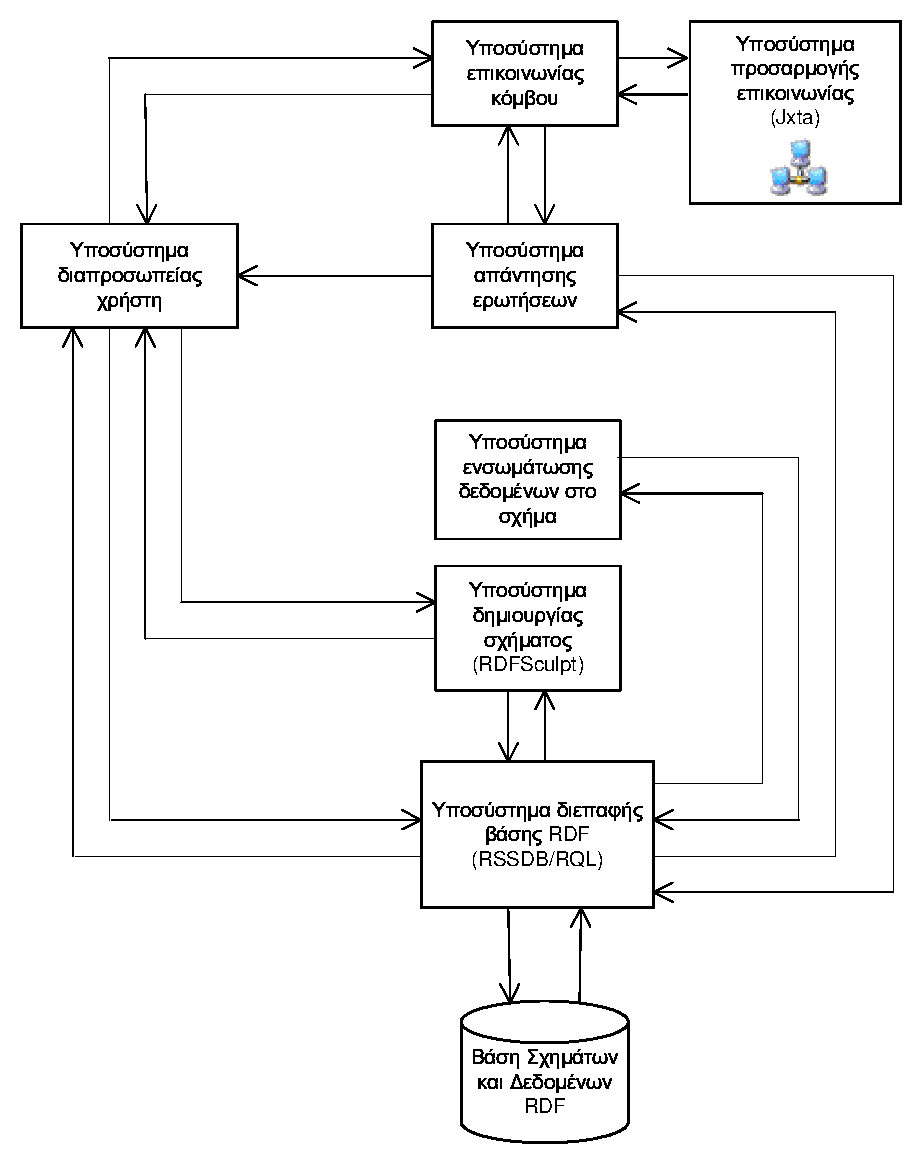
\includegraphics{figures/peerArchitecture.eps} 
    \caption{Αρχιτεκτονική Απλού Κόμβου}
    \label{figure4.1}
\end{figure} 

Το Σχήμα~\ref{figure4.1} απεικονίζει ..............


\subsection{Περιγραφή υποσυστημάτων}
Παρακάτω δίνεται λεπτομερής περιγραφή για καθένα από τα συστήματα
που αναφέραμε. Η περιγραφή αυτή γίνεται με βάση τα διαγράμματα
ροής δεδομένων.

\subsubsection{Υποσύστημα δημιουργίας σχήματος}
Το υποσύστημα αυτό ...............
	\chapter{Υλοποίηση}
\InitialCharacter{Σ}το κεφάλαιο αυτό περιγράφεται η υλοποίηση του συστήματος, με βάση τη μελέτη που παρουσιάστηκε στο προηγούμενο κεφάλαιο. Αρχικά παρουσιάζεται η πλατφόρμα και τα προγραμματιστικά εργαλεία που χρησιμοποιήθηκαν. Στη συνέχεια δίνονται οι λεπτομέρειες υλοποίησης για τους βασικούς αλγορίθμους του συστήματος καθώς και η δομή του κώδικα.

\section{Λεπτομέρειες υλοποίησης}
Στην ενότητα αυτή παρουσιάζονται οι βασικοί αλγόριθμοι που
αναπτύχθηκαν καθώς και λεπτομέρειες σχετικά με την υλοποίηση της
επικοινωνίας των κόμβων.

\subsection{Αλγόριθμοι}

\subsubsection{Αλγόριθμος εισαγωγής δεδομένων}
Όταν ένας κόμβος εισέρχεται για πρώτη φορά στο σύστημα, αρχικά
δημιουργεί το σχήμα που θέλει χρησιμοποιώντας το \en{RDFSculpt}.
Στη συνέχεια................

\noindent\textbf{Παράδειγμα} \\

Έστω ότι ο κόμβος έχει επιλέξει να συμμετέχει στο σύστημα με το \en{RDF} σχήμα που φαίνεται
στο Σχήμα. Έστω επίσης ότι από το \en{SQL} ερώτημα που έχει κάνει στη σχεσιακη
βάση, έχει προκύψει η όψη που φαίνεται στον Πίνακα. Για τις ανάγκες του παραδείγματος θεωρούμε
ότι η όψη αυτή περιέχει μόνο μία εγγραφή.

...........................

\section{Περιγραφή κλάσεων}
Στην ενότητα αυτή δίνεται μια σύντομη περιγραφή των κλάσεων,
των πεδίων και των μεθόδων που τις απαρτίζουν.

\subsection{\en{public class FirstUi}}
\noindent Η κλάση αυτή κατασκευάζει την οθόνη εισαγωγής του χρήστη στο σύστημα.\\

\noindent\textbf{Πεδία}

\begin{itemize}
\item\src{private GridBagLayout blayout} \\
Το \en{layout} για όλα τα \en{Panel}.
\item\src{private GridBagConstraints con} \\
Τα \en{constraints} για το \en{layout}.
\item\src{private Icon arrowR} \\
Εικονίδιο για το κουμπί \en{Next}.
\end{itemize}

\noindent\textbf{Μέθοδοι}

\begin{itemize}
\item\src{public FirstUi()}\\
Ο κατασκευαστής της κλάσης ο οποίος καλεί την \en{createEntryFrame()}.
\item\src{private void createEntryFrame()}\\
Μέθοδος που κατασκευάζει το en{frame}.
\end{itemize}
	\chapter{Έλεγχος}
\InitialCharacter{Σ}το κεφάλαιο αυτό γίνεται ο έλεγχος καλής λειτουργίας του συστήματος.

\section{Μεθοδολογία Ελέγχου}
Ο έλεγχος του συστήματος αυτού πραγματοποιήθηκε με τη χρήση ενός
σεναρίου λειτουργίας. Σύμφωνα με το σενάριο αυτό θεωρούμε ότι στο
σύστημα υπάρχουν τρεις κόμβοι (\en{peer1,peer2,peer3}). Θεωρούμε
επίσης ότι οι κόμβοι \en{peer2} και \en{peer3} έχουν ήδη σχήμα και
δεδομένα. Το σχήμα του \en{peer2} φαίνεται στο
Σχήμα.



Επίσης η τοπολογία του συστήματος έχει ως εξής: ο \en{peer2} είναι
γείτονας του \en{peer1} και ο \en{peer3} γείτονας του \en{peer2}.

Αρχικά λοιπόν θα δημιουργήσουμε σχήμα για τον κόμβο \en{peer1} και
στη συνέχεια θα εισάγουμε σε αυτό δεδομένα εξετάζοντας έτσι την
καλή λειτουργία του υποσυστήματος δημιουργίας σχήματος και του
υποσυστήματος εισαγωγής δεδομένων. Στη συνέχεια από τον κόμβο αυτό
στέλνουμε ερωτήσεις στους υπόλοιπους για τον έλεγχο του
υποσυστήματος απάντησης ερωτήσεων και επικοινωνίας κόμβων.

\section{Αναλυτική παρουσίαση ελέγχου}
Στην ενότητα αυτή παρουσιάζουμε αναλυτικά τον έλεγχο του
συστήματος σύμφωνα με το σενάριο που περιγράφηκε στην προηγούμενη
ενότητα.
	\chapter{Παράδειγμα Πίνακα}

\section{Συμπεράσματα}
Τα συστήματα ομότιμων κόμβων, προκειμένου να υποστηρίζουν πιο
εκφραστικές λειτουργίες αναπαράστασης και αναζήτησης δεδομένων,
εξελίχθηκαν στα συστήματα ομότιμων κόμβων τα οποία βασίζονται στις
τεχνολογίες του Σημασιολογικού Ιστού για την αναπαράσταση των
δεδομένων μέσω σχημάτων που τα περιγράφουν (\en{Schema-based
peer-to-peer systems}).

Συμπερασματικά το σύστημα που αναπτύχθηκε στα πλαίσια αυτής της
διπλωματικής είναι ένα πλήρες σύστημα ομότιμων κόμβων βασισμένο σε
σχήματα, το οποίο καθιστά δυνατή την αναζήτηση της πληροφορίας με
ένα διαφορετικό τρόπο απ' ότι τα προϋπάρχοντα  συστήματα.

\section{Μελλοντικές Επεκτάσεις}
Το σύστημα που αναπτύχθηκε στα πλαίσια αυτής της διπλωματικής
εργασίας θα μπορούσε να βελτιωθεί και να επεκταθεί περαιτέρω,
τουλάχιστον ως προς τρεις κατευθύνσεις. Συγκεκριμένα, αναφέρονται
τα ακόλουθα:

\begin{itemize}
\item Ενσωμάτωση διαδικασίας επιλογής σχήματος με βάση το οποίο ο
κόμβος θα συμμετέχει στο σύστημα. Έτσι όπως έχει σχεδιαστεί το
σύστημα, κάθε κόμβος έχει τη δυνατότητα να δημιουργήσει πολλά
σχήματα και να αποθηκεύσει δεδομένα σε περισσότερα από ένα. Ως
σχήμα του κόμβου (με βάση το οποίο απαντάει τις ερωτήσεις),
θεωρείται το τελευταίο στο οποίο αποθήκευσε δεδομένα. Η δυνατότητα
επιλογής θα του παρείχε περισσότερη ευελιξία.
\item Δυνατότητα αντιστοίχισης δεδομένων τα οποία να μην είναι
αποθηκευμένα σε βάση δεδομένων αλλά σε αρχεία. Η αποδέσμευση από
τη βάση δεδομένων θα έκανε το σύστημα πιο εύκολο στην εγκατάσταση
και τη χρήση.
\item Αξιολόγηση του συστήματος ως προς τη συμπεριφορά του αν
συμμετέχει σε αυτό μεγάλος αριθμός κόμβων \en{(scalability
testing)} και αν χρησιμοποιηθεί ένα πολύ μεγάλο καθολικό σχήμα. H
αξιολόγηση αυτή αφορά την ταχύτητα με την οποία ένας κόμβος
παίρνει απαντήσεις σε μια ερώτηση καθώς και την ποιότητα των
απαντήσεων.
\end{itemize}

%
	\begin{table}[!tb]
		\centering
		\caption{Πίνακας αλήθειας της λογικής συνάρτησης \en{F}}
		\small
		\renewcommand{\arraystretch}{1.3}
		\begin{tabular}{| c | c | c || c |}
			\hline               
		  	\textbf{\en{A}} & \textbf{\en{B}} &  \textbf{\en{C}} &   \textbf{\en{F}} \\
			\hline
				  0 & 0 & 0 & 0  \\
				  0 & 0 & 1 & 0  \\
				  0 & 1 & 0 & 1  \\
				  0 & 1 & 1 & 0  \\	
				  1 & 0 & 0 & 1  \\
				  1 & 0 & 1 & 0  \\
				  1 & 1 & 0 & 1  \\
				  1 & 1 & 1 & 0  \\
		  	\hline
		\end{tabular}
		\label{table07.01}
	\end{table}
%
	\chapter{Παράδειγμα Μαθηματικών Σχέσεων -- Εκφράσεων και Αλγορίθμων}

\section{Συμπεράσματα}
Τα συστήματα ομότιμων κόμβων, προκειμένου να υποστηρίζουν πιο
εκφραστικές λειτουργίες αναπαράστασης και αναζήτησης δεδομένων,
εξελίχθηκαν στα συστήματα ομότιμων κόμβων τα οποία βασίζονται στις
τεχνολογίες του Σημασιολογικού Ιστού για την αναπαράσταση των
δεδομένων μέσω σχημάτων που τα περιγράφουν (\en{Schema-based
peer-to-peer systems}).

Στα συστήματα αυτά κάθε \en{$\displaystyle y=\int_0^1f(x)dx$} \en{$y=\int_0^1f(x)dx$} κόμβος χρησιμοποιεί ένα σχήμα για την \en{$\displaystyle \sum_{i=0}^{100}a_i$}
αναπαράσταση των δεδομένων του. Όμως σε ένα σύστημα ομότιμων
κόμβων, κάθε κόμβος έχει διαφορετικές απαιτήσεις αναπαράστασης
δεδομένων. Επομένως πρέπει να υπάρχει ευελιξία στην επιλογή \en{$\displaystyle \frac{1}{1+x^2}$}
σχήματος. Τα συστήματα που έχουν προταθεί μέχρι τώρα και παρέχουν
αυτή την ευελιξία, για να είναι δυνατή η αναζήτηση πληροφορίας,
απαιτούν την ύπαρξη κανόνων αντιστοίχισης μεταξύ των σχημάτων με
βάση τους οποίους να μετασχηματίζονται οι ερωτήσεις. Όμως δεν
υποστηρίζεται ακόμα αυτόματη δημιουργία και δυναμική ανανέωση των
κανόνων, που είναι απαραίτητα για τα συστήματα ομότιμων κόμβων.
\begin{equation}
	y=\int_0^1f(x)dx
	\label{equation08.01}
\end{equation}

Η συνεισφορά της (\ref{equation08.01}) παρούσας διπλωματικής εργασίας έχει δύο σκέλη. Το
πρώτο αφορά τη δημιουργία ενός πλήρους συστήματος ομότιμων κόμβων
βασισμένο σε σχήματα \en{RDF} το οποίο παρέχει: (α) την υποδομή
για την επικοινωνία των κόμβων,(β) μηχανισμό δημιουργίας σχήματος,
(γ) μηχανισμό ενσωμάτωσης σχεσιακών δεδομένων στο σχήμα με τη
χρήση αντιστοιχίσεων που δημιουργεί ο χρήστης με τη βοήθεια
ειδικής διαπροσωπείας, (δ) ευέλικτη διαπροσωπεία χρήστη για τη
διατύπωση ερωτημάτων και (ε) μηχανισμό απάντησης και επεξεργασίας
ερωτήσεων.

Το δεύτερο σκέλος αφορά το γεγονός ότι το συγκεκριμένο σύστημα
προσφέρει μια σχετική ευελιξία ως προς την επιλογή του σχήματος
από τον κάθε κόμβο, ενώ ταυτόχρονα δίνει τη δυνατότητα
μετασχηματισμού ερωτήσεων χωρίς τη χρήση κανόνων αντιστοίχισης.
Συγκεκριμένα, τα σχήματα των κόμβων αποτελούν
υποσύνολα$-$όψεις$($\en{views}) ενός βασικού σχήματος που
ονομάζεται καθολικό σχήμα. Εκμεταλλευόμενοι λοιπόν το γεγονός ότι
τα σχήματα αυτά είναι συμβατά μεταξύ τους, έχουμε τη δυνατότητα
ελέγχου της ικανοποιησιμότητας μιας ερώτησης και μετατροπής της
όπου χρειάζεται, χρησιμοποιώντας τόσο το σχήμα του κόμβου όσο και
το καθολικό σχήμα.

Συμπερασματικά το σύστημα που αναπτύχθηκε στα πλαίσια αυτής της
διπλωματικής είναι ένα πλήρες σύστημα ομότιμων κόμβων βασισμένο σε
σχήματα, το οποίο καθιστά δυνατή την αναζήτηση της πληροφορίας με
ένα διαφορετικό τρόπο απ' ότι τα προϋπάρχοντα  συστήματα.

\section{Μελλοντικές Επεκτάσεις}
Το σύστημα που αναπτύχθηκε στα πλαίσια αυτής της διπλωματικής
εργασίας θα μπορούσε να βελτιωθεί και να επεκταθεί περαιτέρω,
τουλάχιστον ως προς τρεις κατευθύνσεις. Συγκεκριμένα, αναφέρονται
τα ακόλουθα:

%
\begin{algorithm}[tb]
  \caption{Μετατροπή δεκαδικού αριθμού σε δυαδικό, με τη μέθοδο των διαδοχικών διαιρέσεων με το 2}
  \label{decimal2binary1}
	\begin{algorithmic}
		\Require $X_{(10)}$ \small (\emph{ο δεκαδικός αριθμός προς μετατροπή}) \normalsize
		\Ensure $X_{(2)}$ \small (\emph{η δυαδική αναπαράσταση του Χ}) \normalsize
		\State Θέσε Δ=$X_{(10)}$ \small (\emph{Δ = διαιρετέος}) \normalsize
		\State Θέσε Π=1 \small (\emph{Π = πηλίκο}) \normalsize
		\State Θέσε $X_{(2)}$=<<>> \small (\emph{<<>> ο κενός χαρακτήρας}) \normalsize
		\While{Π$\neq$0}
			\State Διαίρεσε το Δ με το 2 και βρες το πηλίκο Π, και το υπόλοιπο υ.
			\State $X_{(2)}$=υ+$X_{(2)}$ \small (\emph{Τοποθέτησε το υπόλοιπο υ στα αριστερά του $X_{(2)}$}) \normalsize
			\State Θέσε Δ=Π \small (\emph{Το πηλίκο Π τίθεται ως διαιρετέος για την επόμενη διαίρεση}) \normalsize
		\EndWhile
	\end{algorithmic}
\end{algorithm}
%

%
\begin{algorithm}[tb]
  \caption{Κάποιος αλγόριθμος ...}
  \label{some_algorithm}
  \selectlanguage{english}
  \lstset{language=C}
  \begin{lstlisting}
#include <stdio.h>
#define N 10
/* Block
 * comment */
 
int main()
{
    int i;
 
    // Line comment.
    puts("Hello world!");
 
    for (i = 0; i < N; i++)
    {
        puts("LaTeX is also great for programmers!");
    }
 
    return 0;
}
  \end{lstlisting}
 \selectlanguage{greek}
\end{algorithm}
%

\begin{itemize}
\item Ενσωμάτωση διαδικασίας επιλογής σχήματος με βάση το οποίο ο
κόμβος θα συμμετέχει στο σύστημα. Έτσι όπως έχει σχεδιαστεί το
σύστημα, κάθε κόμβος έχει τη δυνατότητα να δημιουργήσει πολλά
σχήματα και να αποθηκεύσει δεδομένα σε περισσότερα από ένα. Ως
σχήμα του κόμβου (με βάση το οποίο απαντάει τις ερωτήσεις),
θεωρείται το τελευταίο στο οποίο αποθήκευσε δεδομένα. Η δυνατότητα
επιλογής θα του παρείχε περισσότερη ευελιξία.
\item Δυνατότητα αντιστοίχισης δεδομένων τα οποία να μην είναι
αποθηκευμένα σε βάση δεδομένων αλλά σε αρχεία. Η αποδέσμευση από
τη βάση δεδομένων θα έκανε το σύστημα πιο εύκολο στην εγκατάσταση
και τη χρήση.
\item Αξιολόγηση του συστήματος ως προς τη συμπεριφορά του αν
συμμετέχει σε αυτό μεγάλος αριθμός κόμβων \en{(scalability
testing)} και αν χρησιμοποιηθεί ένα πολύ μεγάλο καθολικό σχήμα. H
αξιολόγηση αυτή αφορά την ταχύτητα με την οποία ένας κόμβος
παίρνει απαντήσεις σε μια ερώτηση καθώς και την ποιότητα των
απαντήσεων.
\end{itemize}
    \part{Επίλογος}
	\chapter{Επίλογος}

\section{Συμπεράσματα}
Τα συστήματα ομότιμων κόμβων, προκειμένου να υποστηρίζουν πιο
εκφραστικές λειτουργίες αναπαράστασης και αναζήτησης δεδομένων,
εξελίχθηκαν στα συστήματα ομότιμων κόμβων τα οποία βασίζονται στις
τεχνολογίες του Σημασιολογικού Ιστού για την αναπαράσταση των
δεδομένων μέσω σχημάτων που τα περιγράφουν (\en{Schema-based
peer-to-peer systems}).

Στα συστήματα αυτά κάθε κόμβος χρησιμοποιεί ένα σχήμα για την
αναπαράσταση των δεδομένων του. Όμως σε ένα σύστημα ομότιμων
κόμβων, κάθε κόμβος έχει διαφορετικές απαιτήσεις αναπαράστασης
δεδομένων. Επομένως πρέπει να υπάρχει ευελιξία στην επιλογή
σχήματος. Τα συστήματα που έχουν προταθεί μέχρι τώρα και παρέχουν
αυτή την ευελιξία, για να είναι δυνατή η αναζήτηση πληροφορίας,
απαιτούν την ύπαρξη κανόνων αντιστοίχισης μεταξύ των σχημάτων με
βάση τους οποίους να μετασχηματίζονται οι ερωτήσεις. Όμως δεν
υποστηρίζεται ακόμα αυτόματη δημιουργία και δυναμική ανανέωση των
κανόνων, που είναι απαραίτητα για τα συστήματα ομότιμων κόμβων.

Η συνεισφορά της παρούσας διπλωματικής εργασίας έχει δύο σκέλη. Το
πρώτο αφορά τη δημιουργία ενός πλήρους συστήματος ομότιμων κόμβων
βασισμένο σε σχήματα \en{RDF} το οποίο παρέχει: (α) την υποδομή
για την επικοινωνία των κόμβων,(β) μηχανισμό δημιουργίας σχήματος,
(γ) μηχανισμό ενσωμάτωσης σχεσιακών δεδομένων στο σχήμα με τη
χρήση αντιστοιχίσεων που δημιουργεί ο χρήστης με τη βοήθεια
ειδικής διαπροσωπείας, (δ) ευέλικτη διαπροσωπεία χρήστη για τη
διατύπωση ερωτημάτων και (ε) μηχανισμό απάντησης και επεξεργασίας
ερωτήσεων.

Το δεύτερο σκέλος αφορά το γεγονός ότι το συγκεκριμένο σύστημα
προσφέρει μια σχετική ευελιξία ως προς την επιλογή του σχήματος
από τον κάθε κόμβο, ενώ ταυτόχρονα δίνει τη δυνατότητα
μετασχηματισμού ερωτήσεων χωρίς τη χρήση κανόνων αντιστοίχισης.
Συγκεκριμένα, τα σχήματα των κόμβων αποτελούν
υποσύνολα$-$όψεις$($\en{views}) ενός βασικού σχήματος που
ονομάζεται καθολικό σχήμα. Εκμεταλλευόμενοι λοιπόν το γεγονός ότι
τα σχήματα αυτά είναι συμβατά μεταξύ τους, έχουμε τη δυνατότητα
ελέγχου της ικανοποιησιμότητας μιας ερώτησης και μετατροπής της
όπου χρειάζεται, χρησιμοποιώντας τόσο το σχήμα του κόμβου όσο και
το καθολικό σχήμα.

Συμπερασματικά το σύστημα που αναπτύχθηκε στα πλαίσια αυτής της
διπλωματικής είναι ένα πλήρες σύστημα ομότιμων κόμβων βασισμένο σε
σχήματα, το οποίο καθιστά δυνατή την αναζήτηση της πληροφορίας με
ένα διαφορετικό τρόπο απ' ότι τα προϋπάρχοντα  συστήματα.

\section{Μελλοντικές Επεκτάσεις}
Το σύστημα που αναπτύχθηκε στα πλαίσια αυτής της διπλωματικής
εργασίας θα μπορούσε να βελτιωθεί και να επεκταθεί περαιτέρω,
τουλάχιστον ως προς τρεις κατευθύνσεις. Συγκεκριμένα, αναφέρονται
τα ακόλουθα:

\begin{itemize}
\item Ενσωμάτωση διαδικασίας επιλογής σχήματος με βάση το οποίο ο
κόμβος θα συμμετέχει στο σύστημα. Έτσι όπως έχει σχεδιαστεί το
σύστημα, κάθε κόμβος έχει τη δυνατότητα να δημιουργήσει πολλά
σχήματα και να αποθηκεύσει δεδομένα σε περισσότερα από ένα. Ως
σχήμα του κόμβου (με βάση το οποίο απαντάει τις ερωτήσεις),
θεωρείται το τελευταίο στο οποίο αποθήκευσε δεδομένα. Η δυνατότητα
επιλογής θα του παρείχε περισσότερη ευελιξία.
\item Δυνατότητα αντιστοίχισης δεδομένων τα οποία να μην είναι
αποθηκευμένα σε βάση δεδομένων αλλά σε αρχεία. Η αποδέσμευση από
τη βάση δεδομένων θα έκανε το σύστημα πιο εύκολο στην εγκατάσταση
και τη χρήση.
\item Αξιολόγηση του συστήματος ως προς τη συμπεριφορά του αν
συμμετέχει σε αυτό μεγάλος αριθμός κόμβων \en{(scalability
testing)} και αν χρησιμοποιηθεί ένα πολύ μεγάλο καθολικό σχήμα. H
αξιολόγηση αυτή αφορά την ταχύτητα με την οποία ένας κόμβος
παίρνει απαντήσεις σε μια ερώτηση καθώς και την ποιότητα των
απαντήσεων.
\end{itemize}
% Παραρτήματα
	\appendices
	\chapter{Παράδειγμα  Παραρτήματος}

\section{Πρώτη ενότητα}
Τα συστήματα ομότιμων κόμβων, προκειμένου να υποστηρίζουν πιο
εκφραστικές λειτουργίες αναπαράστασης και αναζήτησης δεδομένων,
εξελίχθηκαν στα συστήματα ομότιμων κόμβων τα οποία βασίζονται στις
τεχνολογίες του Σημασιολογικού Ιστού για την αναπαράσταση των
δεδομένων μέσω σχημάτων που τα περιγράφουν (\en{Schema-based
peer-to-peer systems}).

Συμπερασματικά το σύστημα που αναπτύχθηκε στα πλαίσια αυτής της
διπλωματικής είναι ένα πλήρες σύστημα ομότιμων κόμβων βασισμένο σε
σχήματα, το οποίο καθιστά δυνατή την αναζήτηση της πληροφορίας με
ένα διαφορετικό τρόπο απ' ότι τα προϋπάρχοντα  συστήματα.

\section{Μελλοντικές Επεκτάσεις}
Το σύστημα που αναπτύχθηκε στα πλαίσια αυτής της διπλωματικής
εργασίας θα μπορούσε να βελτιωθεί και να επεκταθεί περαιτέρω,
τουλάχιστον ως προς τρεις κατευθύνσεις. Συγκεκριμένα, αναφέρονται
τα ακόλουθα:

\begin{itemize}
\item Ενσωμάτωση διαδικασίας επιλογής σχήματος με βάση το οποίο ο
κόμβος θα συμμετέχει στο σύστημα. Έτσι όπως έχει σχεδιαστεί το
σύστημα, κάθε κόμβος έχει τη δυνατότητα να δημιουργήσει πολλά
σχήματα και να αποθηκεύσει δεδομένα σε περισσότερα από ένα. Ως
σχήμα του κόμβου (με βάση το οποίο απαντάει τις ερωτήσεις),
θεωρείται το τελευταίο στο οποίο αποθήκευσε δεδομένα. Η δυνατότητα
επιλογής θα του παρείχε περισσότερη ευελιξία.
\item Δυνατότητα αντιστοίχισης δεδομένων τα οποία να μην είναι
αποθηκευμένα σε βάση δεδομένων αλλά σε αρχεία. Η αποδέσμευση από
τη βάση δεδομένων θα έκανε το σύστημα πιο εύκολο στην εγκατάσταση
και τη χρήση.
\item Αξιολόγηση του συστήματος ως προς τη συμπεριφορά του αν
συμμετέχει σε αυτό μεγάλος αριθμός κόμβων \en{(scalability
testing)} και αν χρησιμοποιηθεί ένα πολύ μεγάλο καθολικό σχήμα. H
αξιολόγηση αυτή αφορά την ταχύτητα με την οποία ένας κόμβος
παίρνει απαντήσεις σε μια ερώτηση καθώς και την ποιότητα των
απαντήσεων.
\end{itemize}

%
	\begin{table}[!tb]
		\centering
		\caption{Πίνακας αλήθειας της λογικής συνάρτησης \en{F}}
		\small
		\renewcommand{\arraystretch}{1.3}
		\begin{tabular}{| c | c | c || c |}
			\hline               
		  	\textbf{\en{A}} & \textbf{\en{B}} &  \textbf{\en{C}} &   \textbf{\en{F}} \\
			\hline
				  0 & 0 & 0 & 0  \\
				  0 & 0 & 1 & 0  \\
				  0 & 1 & 0 & 1  \\
				  0 & 1 & 1 & 0  \\	
				  1 & 0 & 0 & 1  \\
				  1 & 0 & 1 & 0  \\
				  1 & 1 & 0 & 1  \\
				  1 & 1 & 1 & 0  \\
		  	\hline
		\end{tabular}
		\label{table_appA.01}
	\end{table}
%
	\chapter{Απόδειξη της σχέσης (8.1)}
Στο κεφάλαιο αυτό παρουσιάζεται η μελέτη που έγινε για την
υλοποίηση του συστήματος. Αρχικά περιγράφεται η αρχιτεκτονική του
συστήματος και γίνεται ο διαχωρισμός του στα επιμέρους
υποσυστήματα, ενώ στη συνέχεια περιγράφονται οι εφαρμογές του
συστήματος. \expandafter\textgreek{ελένη}

\section{Ανάλυση - περιγραφή αρχιτεκτονικής}
Στην ενότητα αυτή παρουσιάζεται η ανάλυση του συστήματος και ο
χωρισμός του σε υποσυστήματα όσον αφορά την αρχιτεκτονική.

\subsection{Διαχωρισμός υποσυστημάτων}
Το σύστημα αποτελείται από τους απλούς κόμβους και ένα κόμβο
διαχειριστή. Στο σημείο αυτό αναλύουμε το σύστημα ενός απλού
κόμβου, το οποίο αποτελείται από τα εξής υποσυστήματα:

\begin{itemize}
\item Υποσύστημα δημιουργίας σχήματος.
\item Υποσύστημα ενσωμάτωσης δεδομένων στο σχήμα.
\item Υποσύστημα επικοινωνίας κόμβου.
\end{itemize}


\begin{figure}[!ht] \centering
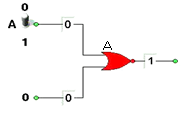
\includegraphics{figures/2.png} \caption{Προσομοίωση Πύλης \en{NOR}}\label{figureB.1}
\end{figure}

Το Σχήμα~\ref{figureB.1} απεικονίζει .................


\subsection{Περιγραφή υποσυστημάτων}
Παρακάτω δίνεται λεπτομερής περιγραφή για καθένα από τα συστήματα
που αναφέραμε. Η περιγραφή αυτή γίνεται με βάση τα διαγράμματα
ροής δεδομένων.

\subsubsection{Υποσύστημα δημιουργίας σχήματος}
Το υποσύστημα αυτό ...............
    \chapter{Παραδείγματα Βιβλιογραφικών Αναφορών}

\begin{center}
	\begin{tabular}{|c|c|}
    	\hline
    	\textbf{Τύπος βιβλιογραφικής πηγής} & \textbf{Αριθμός αναφοράς} \\
    	\hline\hline
    	Βιβλίο ξενόγλωσσο &  \cite{goossens93} \\
    	\hline
    	Βιβλίο ελληνικό &  \cite{greekbook} \\
    	\hline
    	Άρθρο σε επιστημονικό περιοδικό &  \cite{LiArTs13} \\
    	\hline
    	Παρουσίαση σε επιστημονικό συνέδριο &  \cite{dcis2011} \\
    	\hline
    	Ιστοσελίδα &  \cite{LaTeXProject} \\
    	\hline
    	Διπλωματική εργασία &  \cite{zoi04} \\
    	\hline
    	Πτυχιακή εργασία &  \cite{elli05} \\
    	\hline
    	Μεταπτυχιακή διπλωματική εργασία &  \cite{master04} \\
    	\hline
    	Διδακτορική διατριβή &  \cite{phd045} \\
    	\hline
    	Δίπλωμα ευρεσιτεχνίας (πατέντα) &  \cite{viswanathan2014convenient} \\
    	\hline
    	Τεχνική αναφορά &  \cite{MSU-CSE-05-29} \\
    	\hline
    \end{tabular}
\end{center}

          


    \chapter{Δημιουργία Ευρετηρίου}
Δείτε το περιεχόμενο του αρχείου \en{appD.tex} για τρόπους ορισμού ελληνικών και ξενόγλωσσων όρων ευρετηρίου.

% Παραδείγματα ξενόγλωσσων όρων
\indexEN{xerox} \indexEN{babel} \indexEN{anna} \indexEN{babylon}

% Παραδείγματα ελληνικών όρων (προσέξτε τη χρήση λατινικού προθέματος για τη σωστή ταξινόμηση των όρων) 
\indexGR{P@πτυχιακή} \indexGR{E@έλενα} \indexGR{E@ελένη} \indexGR{X@χρώμα} \indexGR{R@ροή} \indexGR{Z@ώριμος} \indexGR{A@άννα} 

    \chapter{Εισαγωγή Εικόνων}
Δείτε το περιεχόμενο του αρχείου \en{appE.tex} για τον τρόπο εισαγωγής εικόνων.

\begin{Illustration}[!h] 
	\centering
	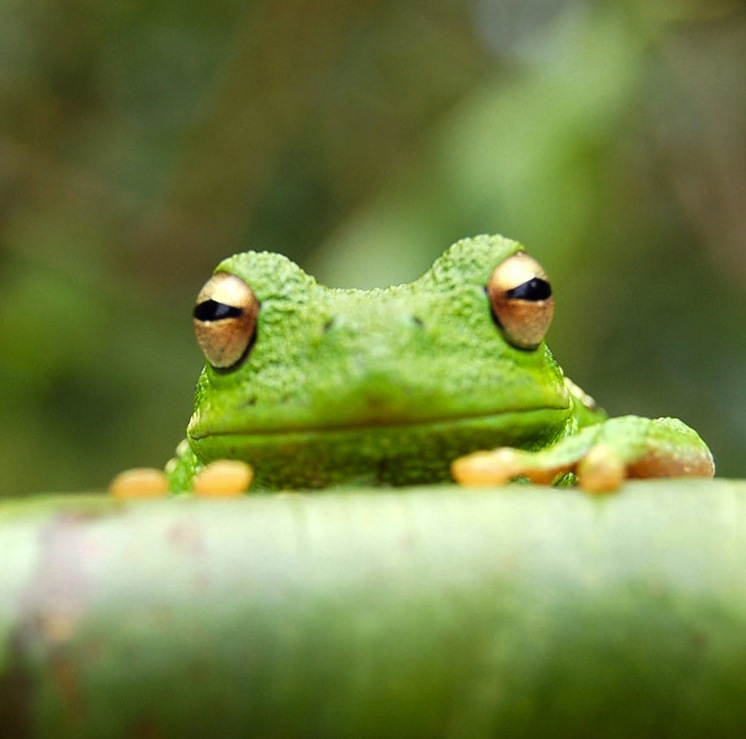
\includegraphics[width=0.5\textwidth]{figures/frog.jpg} 
	\caption{Βάτραχος}
	\label{frog_image}
\end{Illustration}
 
% Βιβλιογραφία - Αναφορές
	\bibliography{references}
% Συντομογραφίες - Αρκτικόλεξα - Ακρωνύμια
	\includeabbreviations{back_matter/abbreviations}
% Γλωσσάριο
	\includeglossary{back_matter/glossary}
%%%%%%%%%%%%%%%%%%%%%%%%%%%%%%%%%%%%%%%%%%%%%%%%%%%%
% Ευρετήριο Όρων
	\printindices
%
%%%%%%%%%%%%%%%%%%
%%%%%%%%%%%%%%%%%%

%% Δημιουργία ετικετών CD:

	\definecdlabeloffsets{0}{-0.65}{0}{0.55} % upper label x offset [cm] (default=0) /  upper label y offset [cm] (default=0) /  lower label x offset [cm] (default=0) /  lower  label y offset [cm] (default=0) -- For Q-Connect KF01579 labels use the following offset values: {0}{-0.65}{0}{0.55}

	\createcdlabel{Πρότυπο Σύστημα Ομότιμων \\ Κόμβων Βασισμένο σε Σχήματα \en{RDF}}{Κωνσταντίνος Δ. Δημητρίου}{ΟΚΤΩΒΡΙΟΣ}{2020}{8} % τίτλος διπλωματικής / όνομα συγγραφέα / μήνας / έτος / εύρος περιοχής τίτλου σε cm (προτεινόμενη τιμή: 8) 

%%σ
%% Δημιουργία εξωφύλλου θήκης CD:

	\createcdcover{Πρότυπο Σύστημα Ομότιμων \\ Κόμβων Βασισμένο σε Σχήματα \en{RDF}}{Στάμος Φ. Ευάγγελος}{ΟΚΤΩΒΡΙΟΣ}{2020}{10} % τίτλος πτυχιακής / όνομα συγγραφέα / μήνας / έτος / εύρος περιοχής τίτλου σε cm (προτεινόμενη τιμή: 10) 

%%
%
\end{document}

%%%%%%%%%%%%%%%%%%%%%%%%%%%%%%%%%%%%%%%%%%%%%%%%%%%%
